\chapterimage{tabl_cont4.pdf} % Chapter heading image

\chapter{Tableau}
\section{Introduzione}
\textbf{Tableau} è una piattaforma avanzata di Business Intelligence, progettata per la visualizzazione interattiva dei dati e l'analisi decisionale. Fondata nel 2003 a Mountain View, California, da un gruppo di ricercatori della Stanford University e attualmente con sede a Seattle, Washington, Tableau offre strumenti potenti per la creazione di Dashboard interattive e personalizzabili, che consentono agli utenti di esplorare, analizzare e condividere i propri dati in tempo reale. Grazie alla sua capacità di integrarsi facilmente con diverse fonti di dati, tra cui file, database relazionali e server, Tableau consente di combinare informazioni eterogenee senza la necessità di conoscenze tecniche avanzate.

\begin{figure}[h!]
    \centering
    
\includegraphics[width=0.4\linewidth]{capitolo_3/img3/Tableau_logo.png}
    \caption{Tableau - Logo}
    \label{fig:Tableau_logo}
\end{figure}

Un elemento distintivo che ha contribuito al successo globale di Tableau è il suo approccio intuitivo all'interazione con i dati, reso possibile dal \textit{VizQL} (\textit{Visual Query Language}), una tecnologia che trasforma in modo semplice e immediato query complesse in visualizzazioni facilmente interpretabili. Questo consente alle aziende di raccogliere, analizzare e visualizzare grandi volumi di dati, rendendo le informazioni più accessibili e utili per decisioni strategiche informate.

La piattaforma supporta modalità di connessione ai dati sia in tempo reale che in memoria, garantendo prestazioni elevate e tempi di risposta rapidi, anche con dataset di dimensioni rilevanti. Le funzionalità di collaborazione in tempo reale e la centralizzazione dei dati tramite Tableau Server assicurano che le organizzazioni possano accedere alle informazioni in modo rapido e sicuro. Questo rende Tableau una soluzione ideale per le imprese che necessitano di una gestione efficiente e sicura dei propri dati, senza compromettere l'usabilità e la velocità nell'analisi.


\subsection{Caricamento dei dati}
Nel software Tableau sono stati caricati i due files: \textbf{FAOSTAT\_data\_1-10-2022}, che contiene dati sui cambiamenti di temperatura, e \textbf{Global Data on Sustainable Energy (2000-2020)}, che raccoglie informazioni relative all’energia sostenibile per diversi paesi dal 2000 al 2020. Prima del caricamento, è stato necessario un processo di uniformazione dei dati relativi agli Stati, poiché i nomi dei Paesi nei due dataset non erano sempre identici. Ad esempio, la denominazione "United States of America" è stata modificata in "United States" in entrambi i file per garantire una corrispondenza univoca. Dopo questa fase di pulizia, i dataset sono stati importati nell’editor Origine dati di Tableau. Per creare un collegamento tra le informazioni provenienti dalle due fonti, è stata stabilita una \textbf{relazione} utilizzando due campi in comune: il campo \texttt{Year}, presente in entrambi i dataset e rappresentante l’anno di riferimento dei dati, e il campo \texttt{Area} nel dataset FAOSTAT, che è stato associato al campo \texttt{Entity} del dataset Global Data on Sustainable Energy, poiché entrambi identificano il nome del paese. L’utilizzo della relazione consente a Tableau di mantenere i dati separati ma collegati, evitando la necessità di unione manuale e garantendo maggiore flessibilità nelle analisi. Infine, è stata verificata la correttezza dell’associazione tra i due dataset attraverso la visualizzazione di anteprime dei dati e la creazione di semplici tabelle di controllo per assicurarsi che le informazioni si allineassero correttamente.

\begin{comment}
Da riprendere:

    Come espresso nell’introduzione iniziale di questa tesina. Attraverso Tableau
 è stato analizzato soltanto il Dataset Healthcare Dataset poiché lo span
 temporale dei suoi dati era grande a sufficienza per generare delle previsioni
 ed analisi ottime.
\end{comment}


\section{Data Analysis}

Per svolgere le analisi proposte, sono state create delle \textbf{Dashboard}, le quali consentono una visualizzazione intuitiva ed efficace per gli utenti che vogliono raggiungere obiettivi di indagine specifici. 

Di seguito verranno presentati i grafici e le analisi ottenute dalle seguenti Dashboard, estratte dai due dataset presi in esame:

\vspace{2mm}
\begin{itemize}
    \item \textbf{Emissioni di CO\textsubscript{2} per Paese in relazione all'area territoriale}
    \item \textbf{Produzione di elettricità rinnovabile in relazione all'area territoriale}
    \item \textbf{Previsione - Emissioni di CO\textsubscript{2}: andamento e proiezioni}
    \item \textbf{Previsione - Produzione di elettricità: andamento e previsioni}
    \item \textbf{Previsione - Variazioni di temperatura: andamento e proiezioni}
\end{itemize}
\vspace{2mm}

\subsection{Emissioni di CO\textsubscript{2} per Paese in relazione all'area territoriale}
\label{cap3_dash_1}
La Dashboard, illustrata in Figura \ref{fig:emissioni_co2}, consente di analizzare in maniera chiara e intuitiva la relazione tra la produzione di CO\textsubscript{2} e l'area geografica occupata dallo Stato di riferimento, mettendo in correlazione questi dati con la variazione media della temperatura registrata nella medesima area.

Per la sua realizzazione, sono stati impiegati e uniti due dataset: \textbf{FAOSTAT Temperature Change} e \textbf{Global Data on Sustainable Energy (2000-2020)}.

\begin{figure}[h!]
    \centering
    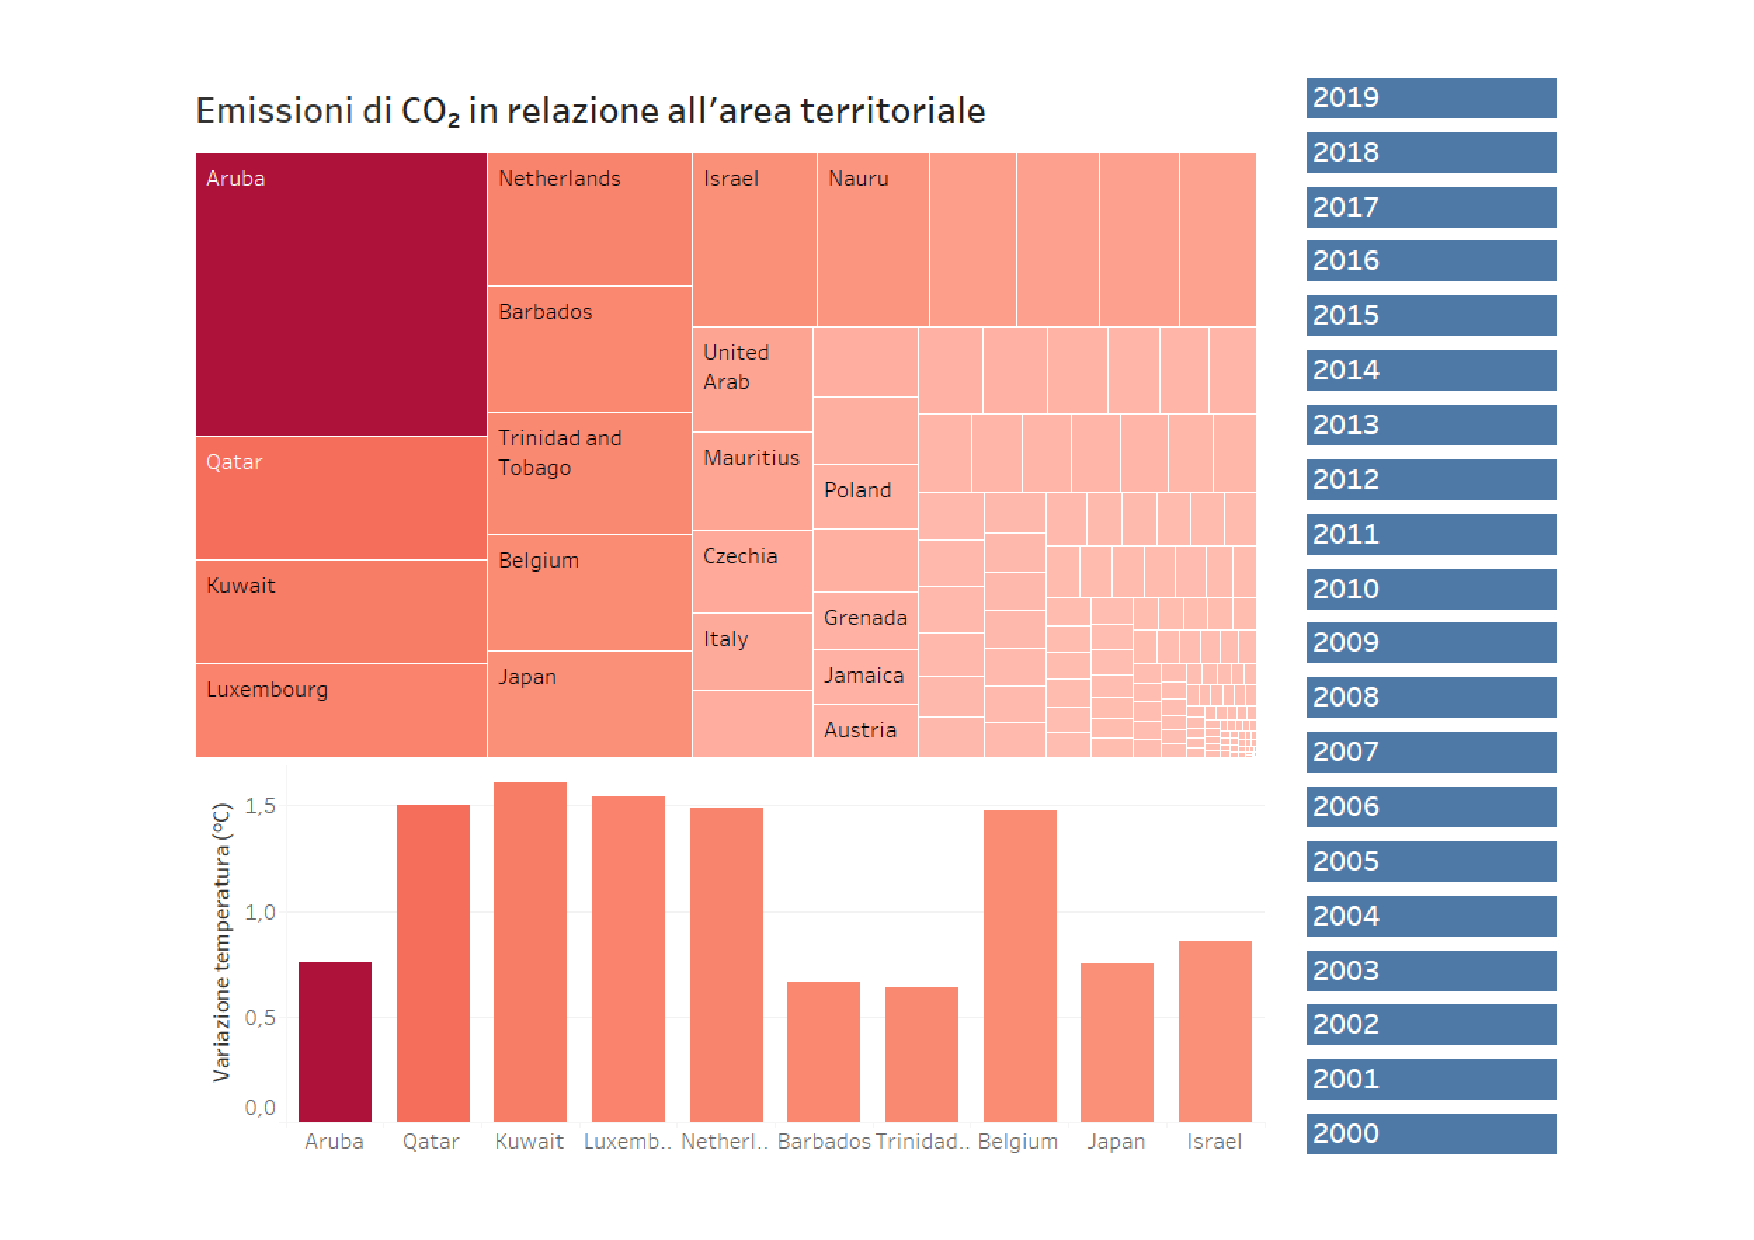
\includegraphics[width=0.98\linewidth]{capitolo_3/img3/Dashboard_CO2_generale_.pdf}
    \caption{Emissioni di CO\textsubscript{2} per Paese in relazione all’area territoriale}
    \label{fig:emissioni_co2}
\end{figure}

\subsubsection{Struttura della Dashboard}
La Dashboard sviluppata in questa sezione è strutturata attorno a due grafici principali, concepiti per offrire un'analisi visiva chiara e approfondita della relazione tra la produzione di emissioni di CO\textsubscript{2} e l'area geografica occupata dai singoli Stati.

Il primo grafico è un \textbf{Treemap}, una rappresentazione visiva gerarchica dei dati che utilizza rettangoli annidati per mostrare le proporzioni relative tra diverse categorie. Questo tipo di visualizzazione è particolarmente utile per evidenziare le differenze dimensionali tra le varie entità e per consentire un confronto immediato dei dati. Nello specifico, il Treemap della Dashboard analizza il rapporto tra la produzione di emissioni di CO\textsubscript{2} e l'estensione territoriale dei diversi Stati. La grandezza di ciascun rettangolo è proporzionale al valore del rapporto: maggiore è l'area del rettangolo, più elevato è il valore dell'indicatore considerato.

Oltre alla dimensione dei rettangoli, il Treemap impiega una scala cromatica basata su diverse sfumature di rosso per fornire un'ulteriore chiave di lettura visiva. Nello specifico, una colorazione più intensa indica un valore più alto del rapporto tra emissioni di CO\textsubscript{2} e area geografica, mentre tonalità più chiare segnalano valori inferiori. Questo approccio consente di cogliere immediatamente le variazioni nei dati e di identificare le aree geografiche con le emissioni più elevate rispetto alla loro estensione territoriale.

Il secondo grafico della Dashboard è un \textbf{Istogramma} che rappresenta la variazione della temperatura media per ciascun Paese.  In particolare la sua struttura è descritta dalle seguenti dimensioni:

\vspace{2mm}
\begin{itemize}
    \item \textit{Asse delle ascisse}: riporta i nomi degli Stati analizzati;
    \item \textit{Asse delle ordinate}: mostra i valori della variazione media di temperatura registrata.
\end{itemize}
\vspace{2mm} 

Le barre sono colorate seguendo la stessa scala cromatica del Treemap, dove tonalità più intense indicano un rapporto più elevato tra emissioni di CO\textsubscript{2} e area geografica. Questa coerenza visiva consente di individuare rapidamente possibili correlazioni tra emissioni e cambiamenti climatici, offrendo un'analisi chiara e intuitiva.

Nella parte destra della Dashboard è presente un filtro, che consente di selezionare gli Anni di interesse, i quali vanno dal 2000 al 2019. Grazie a questa funzionalità interattiva, l'utente può selezionare uno specifico anno e visualizzare i grafici aggiornati.

\subsubsection{Obiettivo dell'Analisi}
La Dashboard si pone come uno strumento utile per effettuare diverse tipologie di analisi, focalizzate sull'esplorazione e la comprensione della relazione tra produzione di emissioni di CO\textsubscript{2}, l'estensione geografica degli Stati e le variazioni di temperatura media, con l'obiettivo di fornire spunti utili sul cambiamento climatico e sull'impatto delle emissioni di CO\textsubscript{2}.

Prendendo in considerazione il grafico Treemap, si osserva che una maggiore dimensione territoriale non comporta necessariamente una produzione maggiore di emissioni di CO\textsubscript{2}. Ad esempio, Paesi come il Giappone e la Polonia, che vantano un'estensione geografica significativa, superiore ai $300.000  \text{km}^2$\footnote{I valori relativi all'area geografica sono stati tratti dal parametro \texttt{Land Area}, presente nel dataset \textit{Global Data on Sustainable Energy (2000-2020)}, il quale esprime la superficie totale del territorio, espressa in chilometri quadrati.}, presentano valori di emissioni ben inferiori rispetto a Stati come Aruba, che, pur avendo una superficie di soli $180  \text{km}^2$, si colloca ai vertici della classifica delle emissioni. Questo confronto evidenzia come la produzione di CO\textsubscript{2} non dipenda esclusivamente dalla dimensione territoriale, ma sia invece influenzata principalmente dal tipo di fonti energetiche utilizzate e dalle politiche ambientali adottate.

Inoltre, analizzando i risultati del secondo grafico, emerge chiaramente che un aumento della produzione di CO\textsubscript{2} da parte di uno Stato non corrisponde necessariamente a un incremento proporzionale della temperatura media locale. Questo osservazione sottolinea come il cambiamento climatico non sia un fenomeno limitato o determinato esclusivamente dalle caratteristiche locali di un singolo paese, ma piuttosto un processo globale che coinvolge l'intero pianeta. Sebbene le emissioni di gas serra siano certamente un fattore chiave, l'effetto del riscaldamento globale si manifesta su scala mondiale, con impatti che vanno ben oltre i confini nazionali, influenzando in maniera complessa e interconnessa le condizioni climatiche a livello globale.

Applicando i filtri relativi agli anni, come illustrato nella Figura \ref{emissioni_co2_1}, l'utente può osservare le dinamiche temporali dei rapporti tra emissioni di CO\textsubscript{2} e superficie territoriale, nonché le fluttuazioni delle temperature medie nel corso del tempo. Questo approccio consente di analizzare come tali variabili si siano evolute, mettendo in evidenza possibili correlazioni tra l'andamento delle emissioni e i cambiamenti climatici. Inoltre, offre l'opportunità di riflettere sull'impatto delle politiche ambientali, economiche e industriali adottate in ciascun periodo, evidenziando come queste possano aver influenzato l'evoluzione dei fenomeni osservati. 

La selezione degli anni \textbf{2000}, \textbf{2010} e \textbf{2019} è stata effettuata al fine di facilitare un confronto diretto con le analisi precedentemente svolte, permettendo così di evidenziare in modo più chiaro le tendenze e le evoluzioni nel tempo.

\begin{myoutline}
     \textbf{Nota}: Selezionando determinati anni, come ad esempio il 2000, è possibile che alcuni Stati non vengano visualizzati nell'istogramma. Questo accade a causa dell'assenza di dati di rilevazione per tali Stati in quel periodo specifico.
\end{myoutline}


\begin{figure}[p]
    \centering
    \subfloat[\textbf{Anno 2000}]{%
        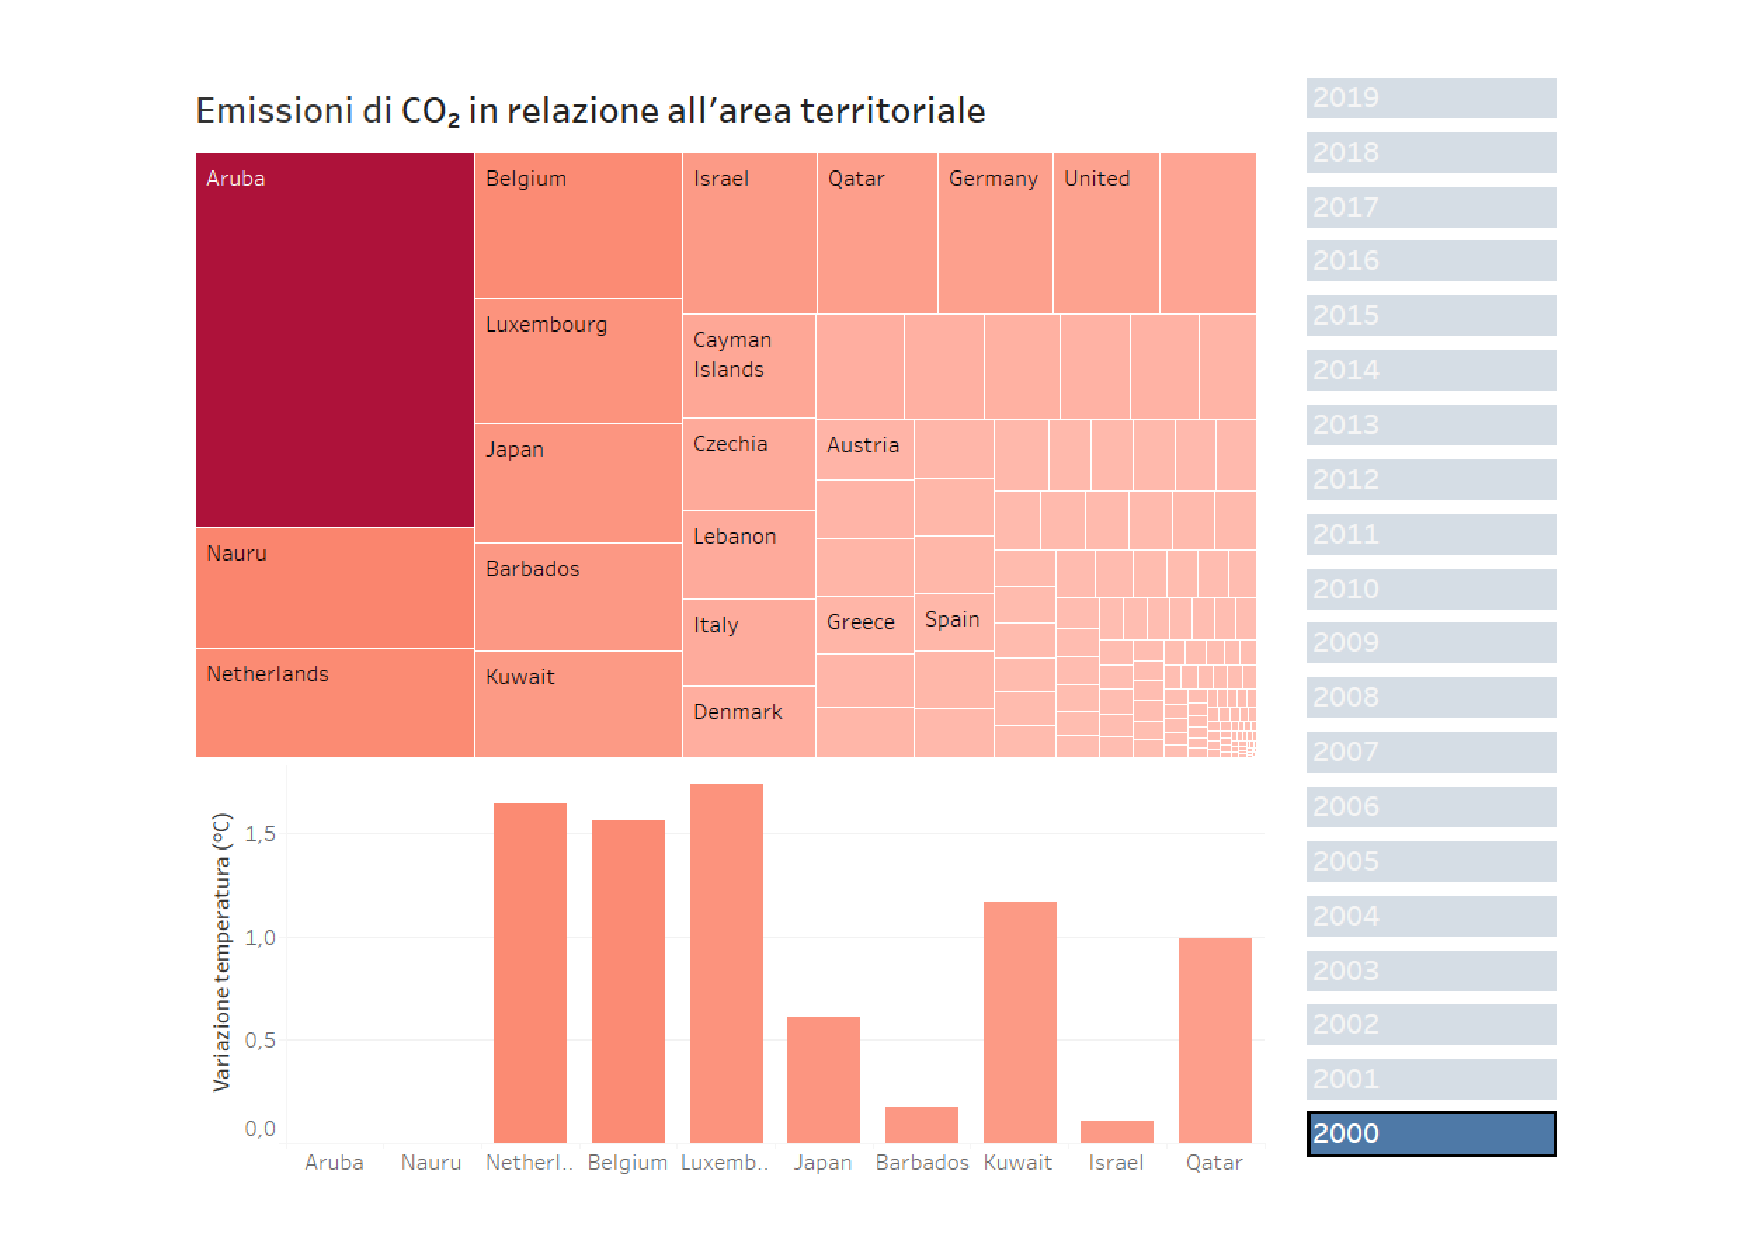
\includegraphics[width=0.7\textwidth]{capitolo_3/img3/Dashboard_CO2_Anno_2000.pdf}}\\
    \subfloat[\textbf{Anno 2010}]{%
        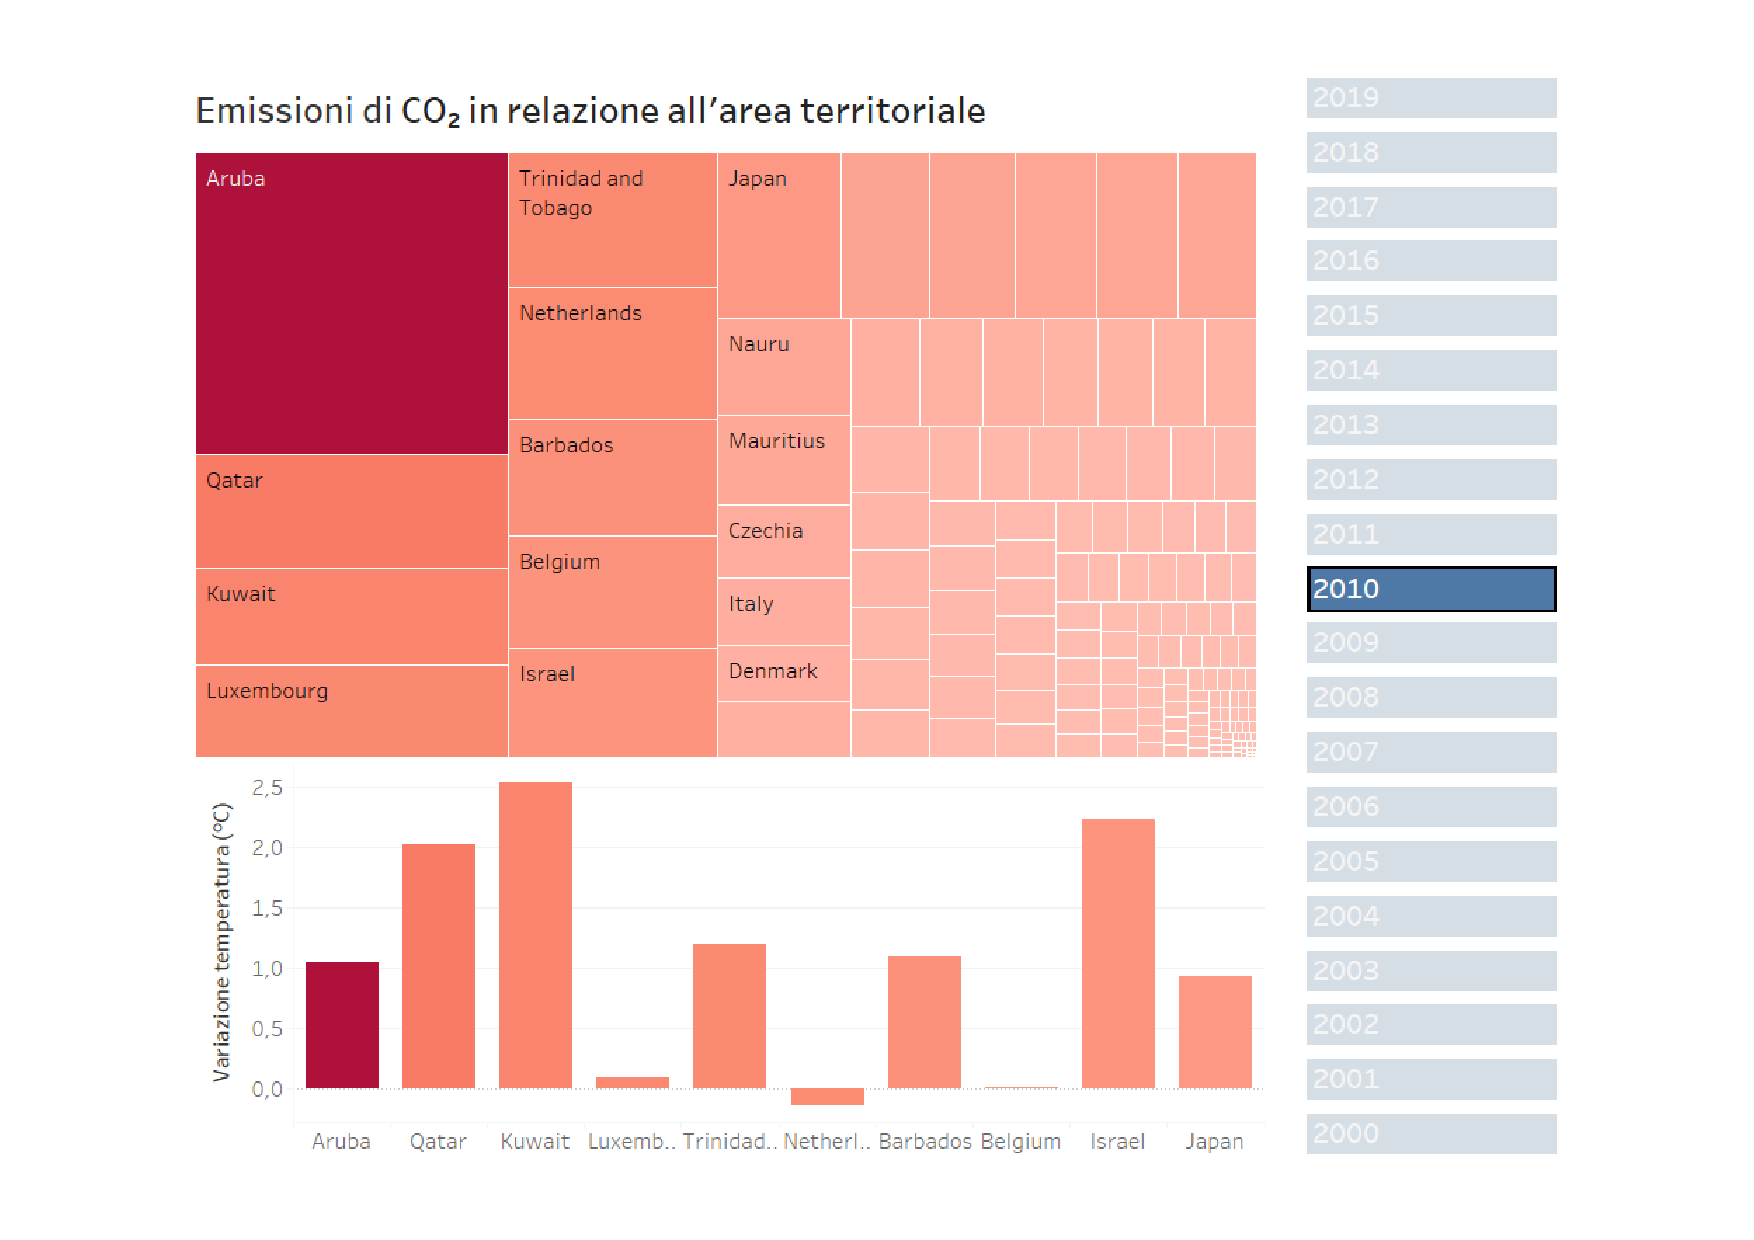
\includegraphics[width=0.7\textwidth]{capitolo_3/img3/Dashboard_CO2_Anno_2010.pdf}} \\
    \subfloat[\textbf{Anno 2019}]{%
        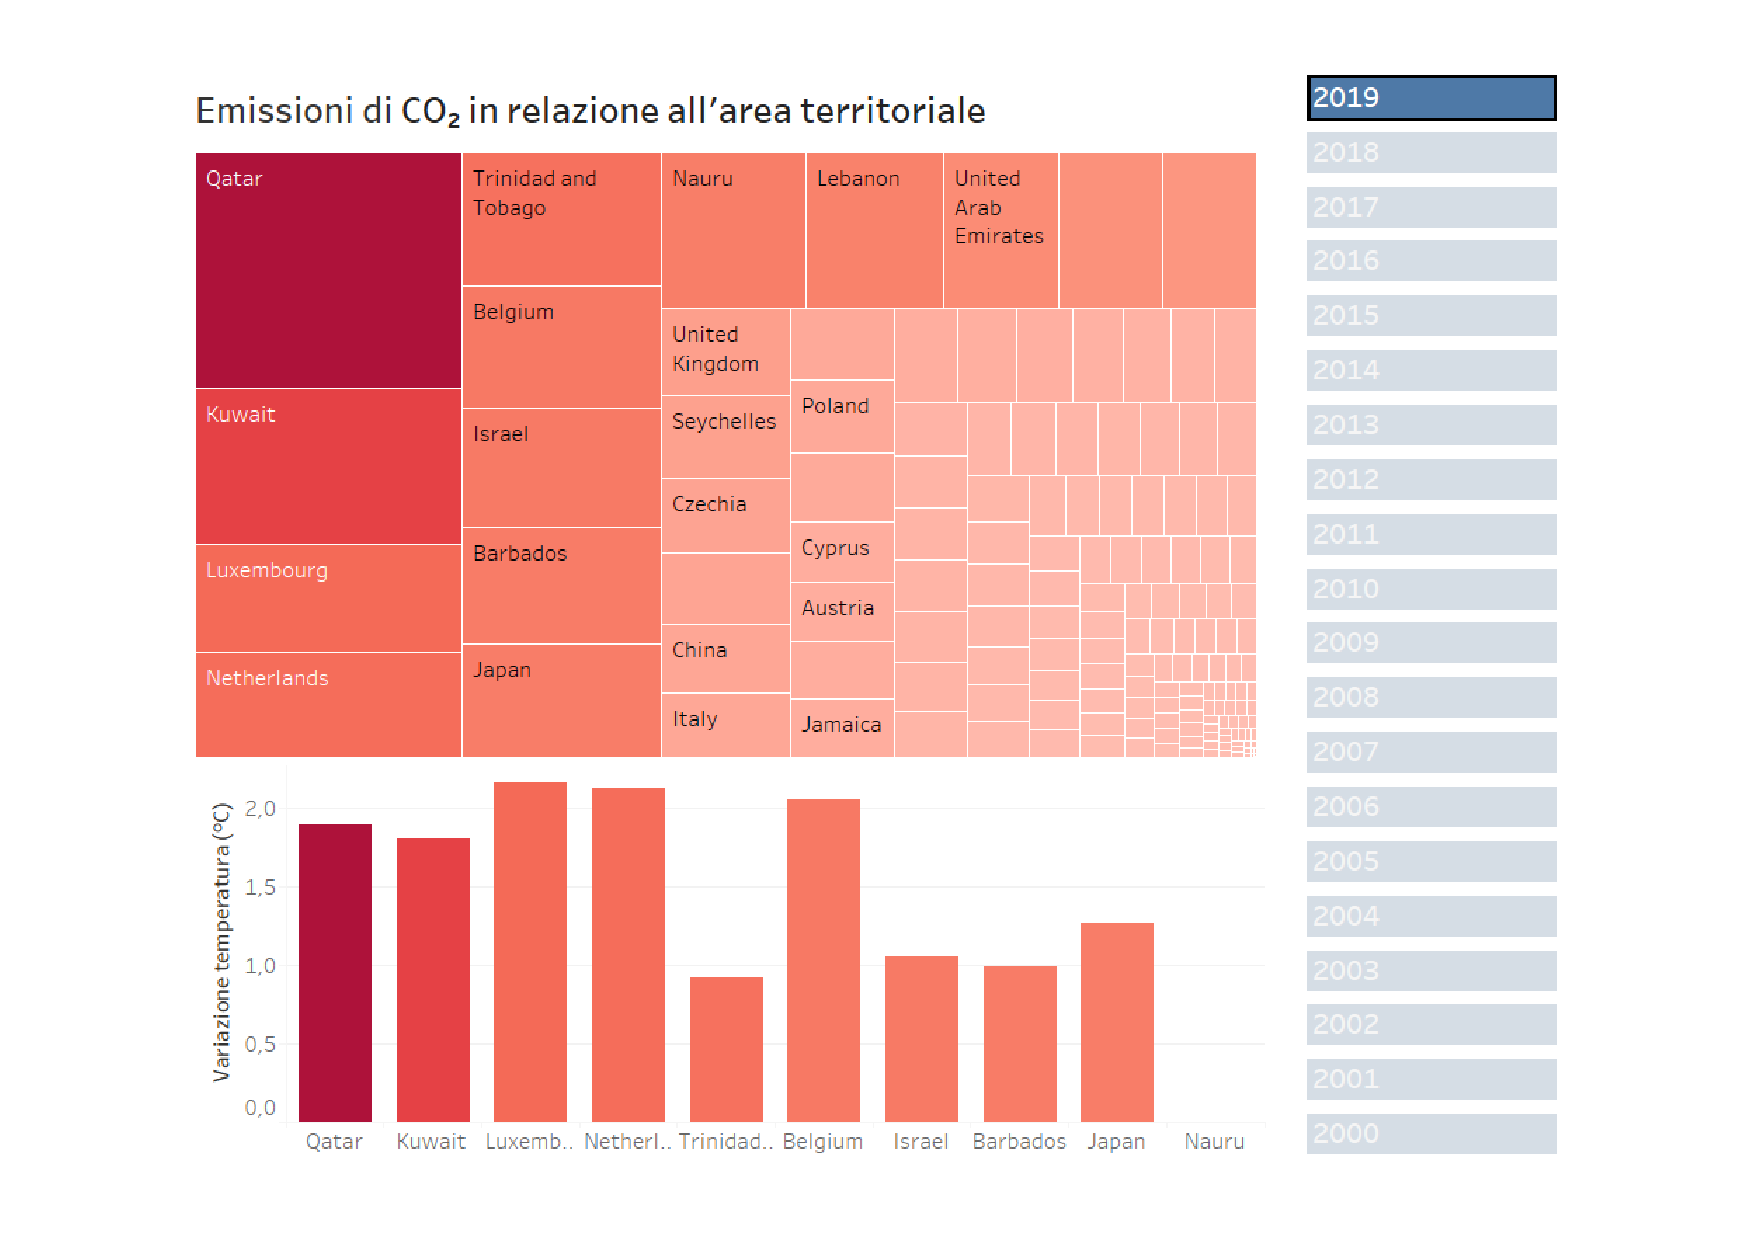
\includegraphics[width=0.7\textwidth]{capitolo_3/img3/Dashboard_CO2_Anno_2019.pdf}}

   \caption{Emissioni di CO\textsubscript{2} per Paese in relazione all'area territoriale - Anno 2000, 2010, 2019}
  \label{emissioni_co2_1}
\end{figure}

\newpage
\subsection{Produzione di elettricità rinnovabile in relazione all'area territoriale}

La Dashboard, illustrata nella Figura \ref{fig:rinnovabile}, fornisce una panoramica dettagliata sulla produzione di energia elettrica da fonti rinnovabili in relazione all'area territoriale.

\begin{figure}[h!]
    \centering
    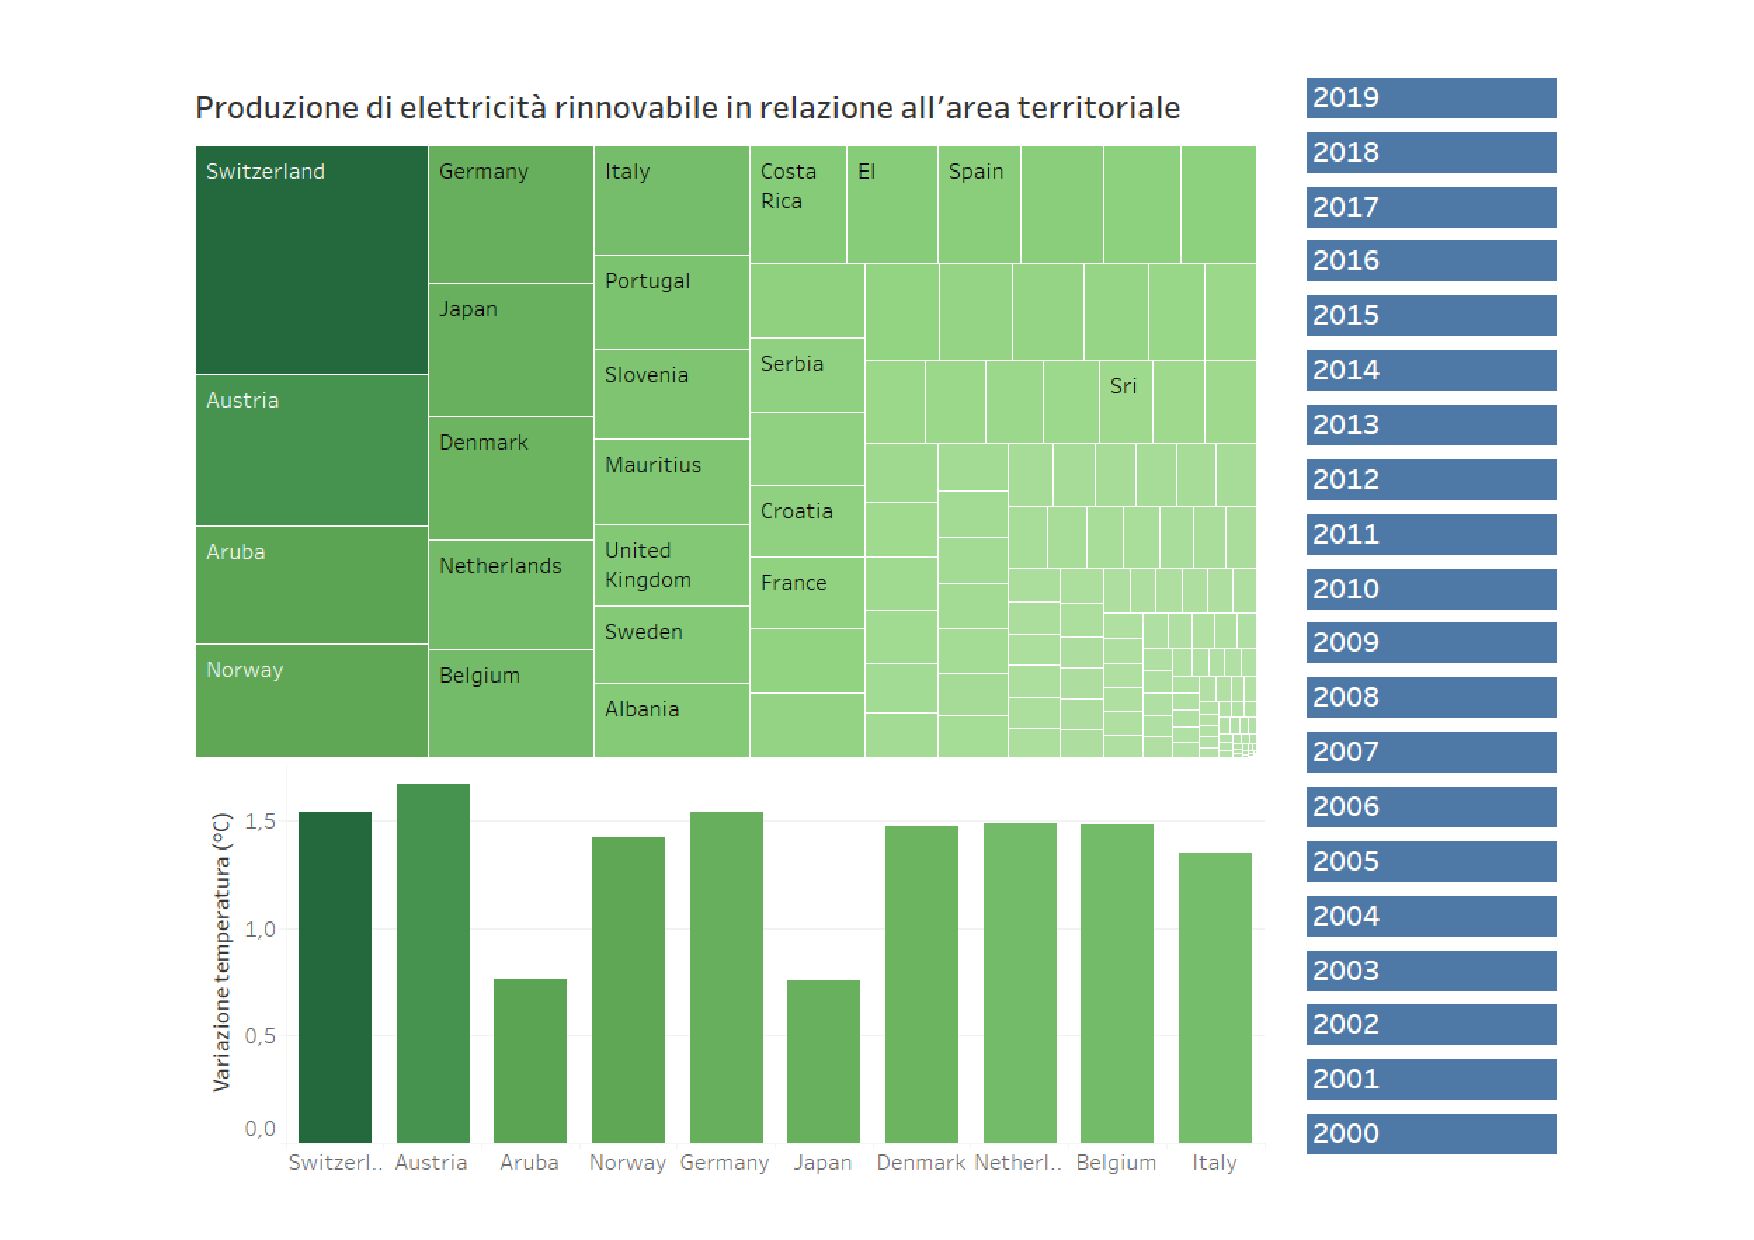
\includegraphics[width=0.98\linewidth]{capitolo_3/img3/Dashboard_Rinnovabile_generale.pdf}
    \caption{Produzione di elettricità rinnovabile in relazione all'area territoriale}
    \label{fig:rinnovabile}
\end{figure}

Per la sua realizzazione, sono stati impiegati e uniti due dataset: \textbf{FAOSTAT Temperature Change} e \textbf{Global Data on Sustainable Energy (2000-2020)}.

\subsubsection{Struttura della Dashboard}

La struttura di questa Dashboard è molto simile a quella presentata nella Sezione \ref{cap3_dash_1}. L'utilizzo degli stessi tipi di grafici ha permesso un confronto più immediato e intuitivo dei risultati ottenuti.

Il primo grafico, \textbf{Treemap}, rappresenta il rapporto tra la produzione di energia elettrica da fonti rinnovabili e l'area territoriale dei diversi Stati analizzati. La dimensione di ciascun rettangolo è proporzionale al valore di tale rapporto: maggiore è l'area del rettangolo, più elevato risulta l'indicatore considerato.  

Oltre alla dimensione dei rettangoli, il Treemap utilizza una scala cromatica basata su diverse sfumature di verde per fornire un'ulteriore chiave di lettura visiva. Nello specifico, tonalità più intense indicano un valore più elevato del rapporto tra produzione di energia rinnovabile ed estensione territoriale, mentre sfumature più chiare rappresentano valori inferiori. Questo approccio consente di cogliere immediatamente le variazioni nei dati e di identificare le aree geografiche con una maggiore incidenza della produzione di energia rinnovabile rispetto alla superficie territoriale.  

Il secondo grafico, un \textbf{Istogramma}, mostra la variazione di temperatura media per ciascun Paese analizzato. Le barre sono colorate secondo la stessa scala cromatica adottata nel Treemap: tonalità più intense indicano un rapporto più elevato tra produzione di energia rinnovabile ed estensione geografica, facilitando così un confronto visivo più intuitivo e coerente tra i due grafici.  

A destra dei grafici è presente un filtro interattivo che consente la selezione degli anni di interesse, coprendo il periodo compreso tra il 2000 e il 2019.

\subsubsection{Obiettivo dell'Analisi}

La Dashboard si configura come uno strumento efficace per condurre diverse tipologie di analisi sulla relazione tra la produzione di energia elettrica da fonti rinnovabili e l'estensione geografica degli Stati considerati. Grazie alla combinazione di visualizzazioni grafiche intuitive, essa consente di individuare tendenze e correlazioni significative, facilitando un'interpretazione immediata e approfondita dei dati.  

Dall'analisi dei grafici emerge chiaramente che la produzione di energia rinnovabile non dipende esclusivamente dall'estensione territoriale di un Paese, bensì dal suo livello di sviluppo industriale e tecnologico. In particolare, si osserva che i Paesi maggiormente rappresentati nella Dashboard appartengono prevalentemente all'Europa, mentre economie di vasta estensione, come gli Stati Uniti e la Cina, risultano assenti. Ciò suggerisce che la transizione verso le energie rinnovabili non sia necessariamente correlata alla disponibilità di ampie superfici territoriali, ma piuttosto a politiche energetiche mirate, investimenti in innovazione e infrastrutture avanzate.  

Un ulteriore aspetto rilevante è la relazione tra la produzione di energia rinnovabile e la variazione della temperatura media. Dai dati dell'Istogramma emerge, infatti, che gli Stati con una maggiore produzione di energia rinnovabile registrano anche un incremento significativo della temperatura media. Questo fenomeno potrebbe essere attribuito a diversi fattori, tra cui il cambiamento climatico globale e le specifiche condizioni ambientali dei Paesi considerati. L'analisi congiunta di questi elementi consente di approfondire le dinamiche in atto e di valutare l'efficacia delle politiche energetiche nel contrastare i cambiamenti climatici.  

Attraverso l'applicazione dei filtri temporali, come illustrato in Figura \ref{rinnovabile_1}, l'utente ha la possibilità di esaminare l'evoluzione della produzione di energia rinnovabile e della superficie territoriale nel tempo, nonché di monitorare le fluttuazioni della temperatura media. Tali filtri permettono non solo di osservare le variazioni nei parametri analizzati, ma anche di valutare l'impatto delle politiche ambientali, economiche e industriali adottate nei diversi periodi. Questo approccio consente di evidenziare in che modo le strategie messe in atto abbiano influenzato i fenomeni osservati.  

In particolare, la selezione degli anni \textbf{2000}, \textbf{2010} e \textbf{2019} è stata effettuata per facilitare un confronto diretto con le analisi precedentemente svolte, permettendo di evidenziare in modo più chiaro le tendenze e le evoluzioni nel tempo. Si osserva, infatti, che nel 2010 le politiche ambientali orientate alla produzione di energia rinnovabile hanno portato a miglioramenti significativi nella variazione della temperatura media, in particolare in Paesi come Norvegia e Danimarca. Tuttavia, nel 2019 tutti gli Stati analizzati hanno registrato un incremento significativo della temperatura, suggerendo che le strategie adottate fino a quel momento non siano state sufficienti per contrastare efficacemente il riscaldamento globale.

\begin{figure}[p]
    \centering
    \subfloat[\textbf{Anno 2000}]{%
        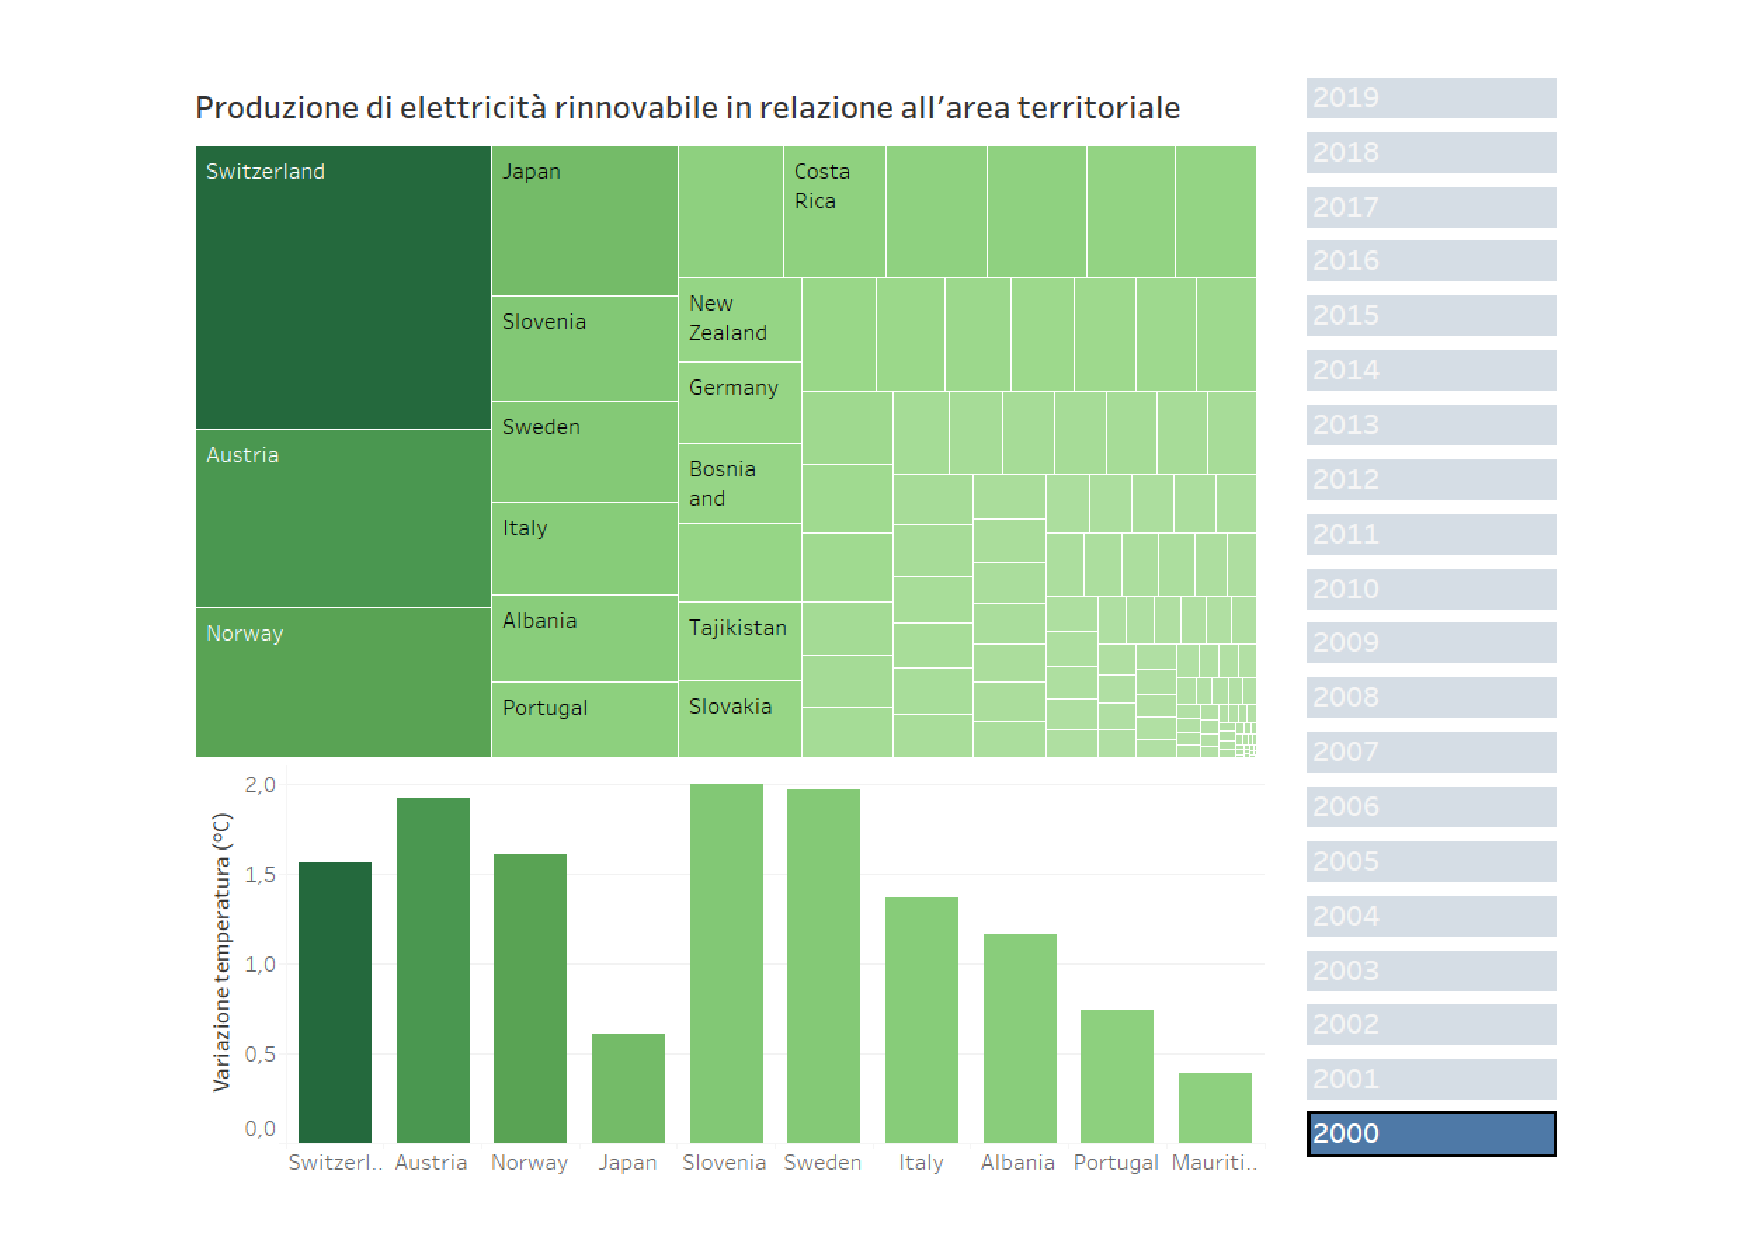
\includegraphics[width=0.7\textwidth]{capitolo_3/img3/Dashboard_Rinnovabile_Anno_2000.pdf}}\\
    \subfloat[\textbf{Anno 2010}]{%
        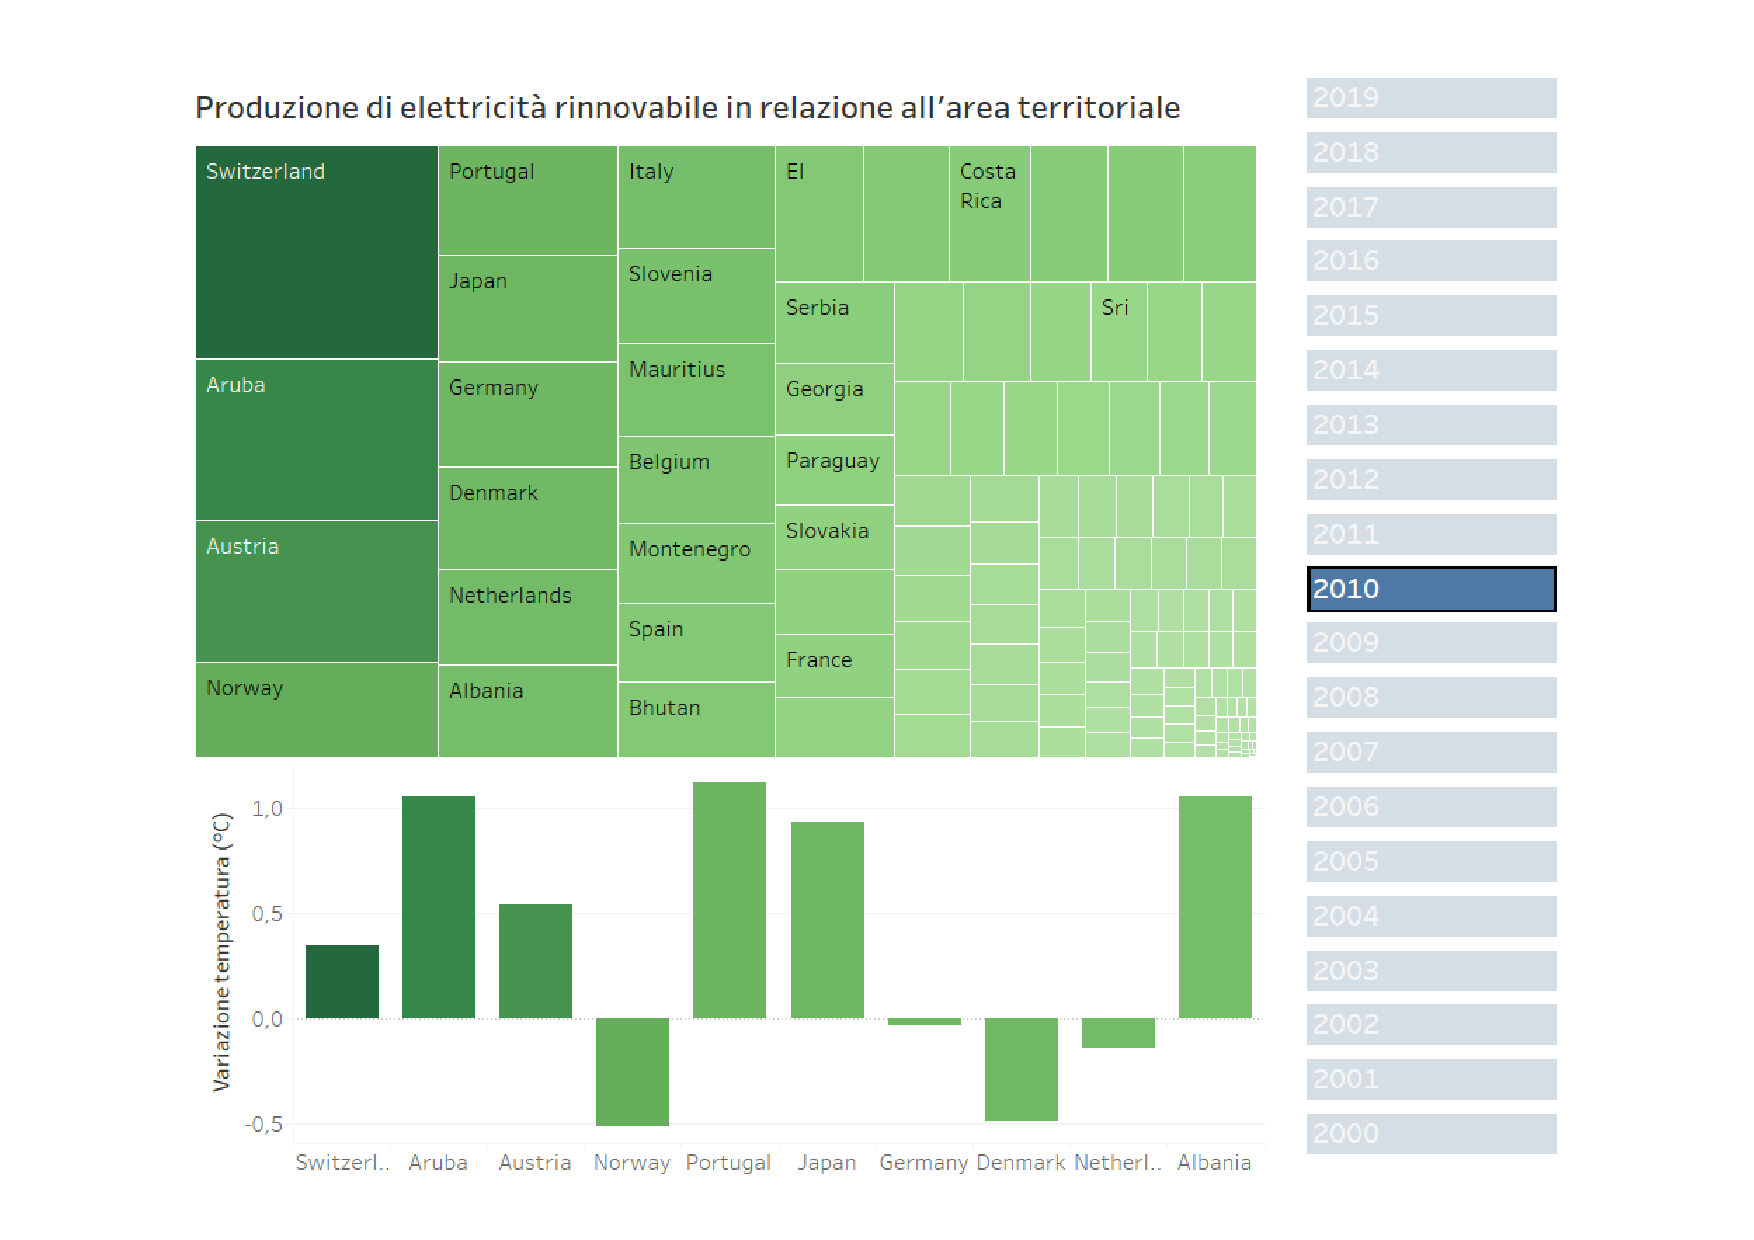
\includegraphics[width=0.7\textwidth]{capitolo_3/img3/Dashboard_Rinnovabile_Anno_2010.pdf}} \\
    \subfloat[\textbf{Anno 2019}]{%
        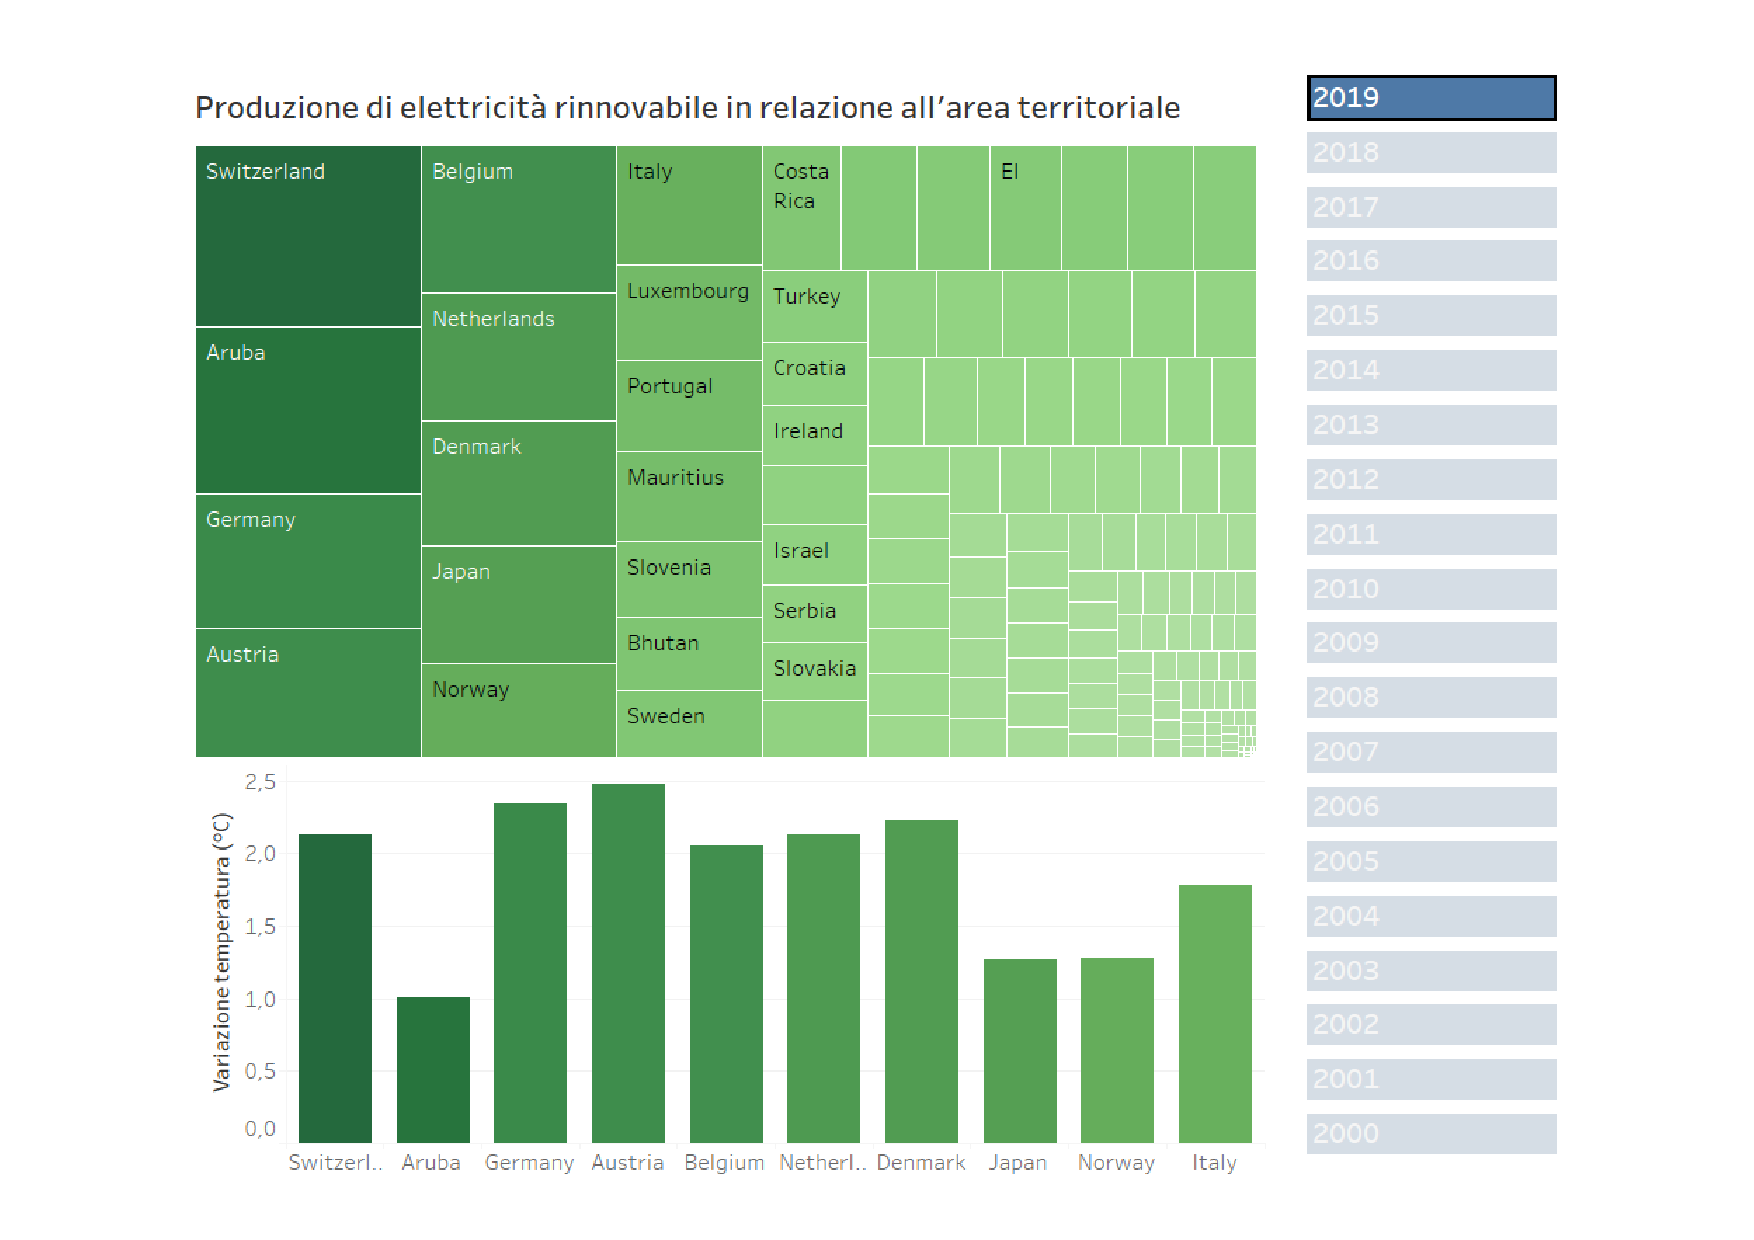
\includegraphics[width=0.7\textwidth]{capitolo_3/img3/Dashboard_Rinnovabile_Anno_2019.pdf}}

   \caption{Produzione di elettricità rinnovabile in relazione all'area territoriale - Anno 2000, 2010, 2019}
  \label{rinnovabile_1}
\end{figure}

\newpage
\subsection{Previsione - Emissioni di CO\textsubscript{2}: andamento e proiezioni}
La Dashboard, illustrata in Figura \ref{fig:previsione_1}, presenta una struttura significativamente differente rispetto a quelle analizzate nelle sezioni precedenti. Mentre le Dashboard precedenti si limitavano all'estrazione e alla visualizzazione di informazioni direttamente derivate dai dataset di riferimento, la presente soluzione si distingue per l'integrazione di un modello predittivo.

\begin{myoutline}
 Le \textbf{Previsioni} permettono di stimare dati futuri basandosi su quelli esistenti. Utilizzando modelli matematici, Tableau analizza i trend e sceglie automaticamente il metodo migliore per creare una previsione accurata. Questo strumento è utile per individuare andamenti e fare ipotesi informate su cosa potrebbe accadere in futuro. Il modello di previsione utilizzato per tutte le visualizzazioni è di tipo Personalizzato con Tendenza e Stagione impostati ad "Aggiuntivo".
\end{myoutline}

La previsione è mostrata utilizzando una funzionalità di Tableau chiamata \textbf{Story}.

\begin{myoutline}
    Le \textbf{Story} sono sequenze di Dashboard e grafici struttura che consentono di creare una narrazione interattiva basata sui dati.
\end{myoutline}

Nello specifico, questa Story visualizza un grafico che rappresenta l'andamento storico (\textit{Change Over Time}) delle emissioni di CO\textsubscript{2} dal 2000 al 2019, integrato con una proiezione delle emissioni future fino al 2026. 
Per la realizzazione di tutte le previsioni, comprese quelle successive, sono stati impiegati e uniti due dataset: \textbf{FAOSTAT Temperature Change} e \textbf{Global Data on Sustainable Energy (2000-2020)}\footnote{Per le previsioni sono stati presi in considerazione i decenni compresi tra il 2000 e il 2019, poiché l'ampiezza dell'intervallo temporale dei dati era sufficientemente estesa da garantire analisi accurate e previsioni affidabili.}.

\begin{figure}[h!]
    \centering
    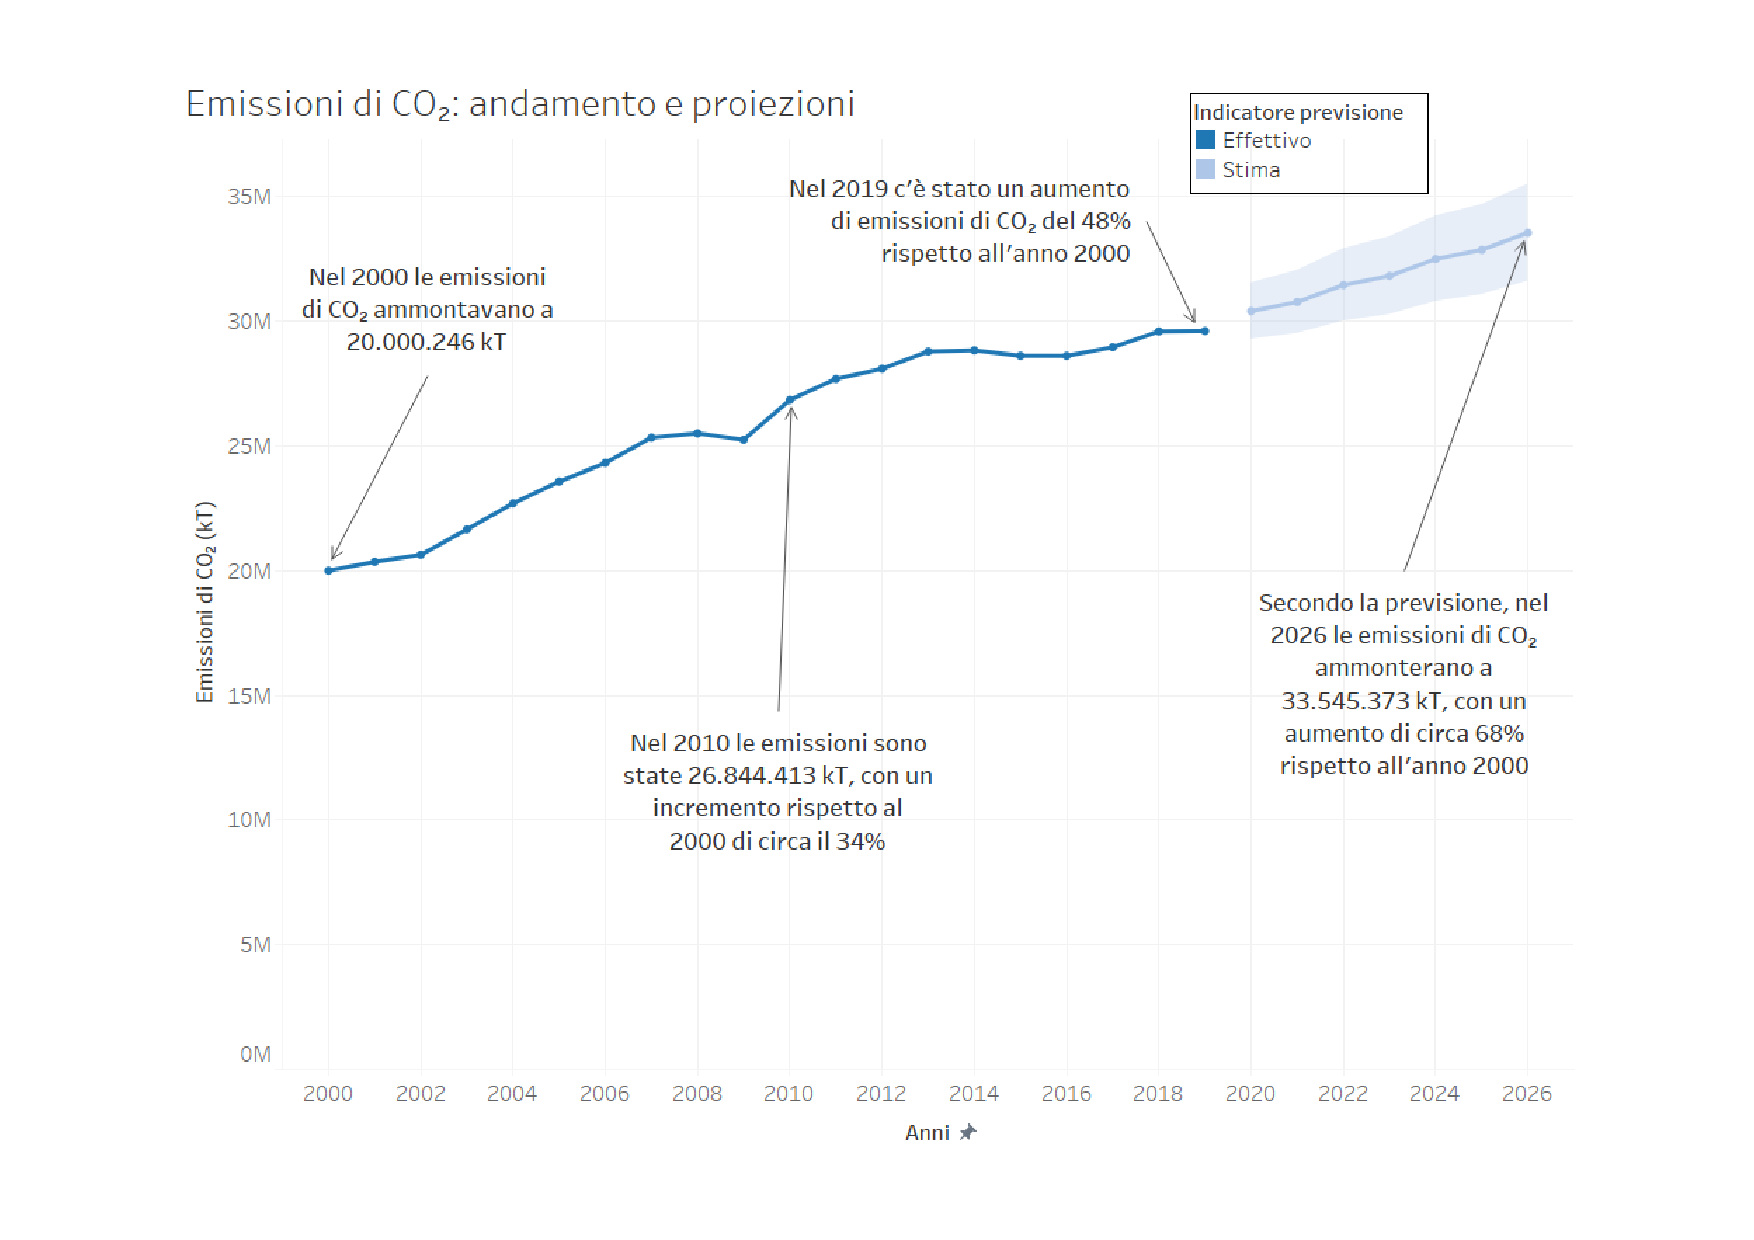
\includegraphics[width=0.98\linewidth]{capitolo_3/img3/previsioni/Dashboard_Previsione_CO2.pdf}
    \caption{Previsione - Emissioni di CO\textsubscript{2}: andamento e proiezioni}
    \label{fig:previsione_1}
\end{figure}

\subsubsection{Risultati della previsione}
Il grafico in Figura \ref{fig:previsione_1} mostra un grafico a linea la cui struttura è delineata dalle seguenti dimensioni: 

\vspace{2mm}
\begin{itemize}
    \item \textit{Asse delle ascisse}: riporta gli anni che vanno dal 2000 al 2026;
    \item \textit{Asse delle ordinate}: mostra i valori delle emissioni di CO\textsubscript{2}, espressi in \texttt{kT}.
\end{itemize}
\vspace{2mm} 

All'interno della \textbf{Story} sono incluse una \textbf{legenda} e delle \textbf{descrizioni}, associate ai principali punti critici del grafico, al fine di agevolare una navigazione più intuitiva e immediata per l'utente.  

L'analisi si concentra sui dati relativi al periodo 2020-2026, che rappresentano i risultati della previsione. Tali dati, ottenuti dall'andamento delle misure presenti nei dataset di riferimento, evidenziano una crescita costante del livello di emissioni di CO\textsubscript{2}. In particolare, come indicato nella descrizione presente all'interno della Dashboard, si prevede un aumento delle emissioni pari a circa il 68\% rispetto ai valori registrati nell'anno 2000.

\begin{myoutline}
Secondo il rapporto del \textit{Global Carbon Project riportato dall'Organizzazione Meteorologica Mondiale} (\textit{OMM})\footnote{\textit{UNRIC (2024). Record 2024 di emissioni di carbonio da combustibili fossili. Organizzazione Meteorologica Mondiale (OMM)}.}, nel 2024 le emissioni totali di anidride carbonica (CO\textsubscript{2}) hanno raggiunto un record storico di 41,6 miliardi di tonnellate. Questa fonte evidenzia come i risultati dell'analisi siano coerenti con il trend osservato nelle misure effettivamente registrate nella realtà, sebbene risultino sottostimati.
\end{myoutline}

Nelle Figure \ref{fig:previsione_1_stati}, sono presenti delle previsioni sempre relative alle emissioni di CO\textsubscript{2}, ma filtrate per ogni specifico Stato. La \textbf{struttura delle Dashboard} si articola in questo modo: 
\vspace{2mm}
\begin{itemize}
    \item \textit{Grafico a linee}: grafico a linee che illustra i risultati della previsione;
    \item \textit{Mappa dello Stato}: visualizzazione geografica per un'interpretazione più intuitiva della Dashboard;
    \item \textit{KPI}: espressioni testuali che riportano il \textit{Nome dello Stato}, il \textit{Valore delle Emissioni di CO\textsubscript{2} previsto per il 2026} e la \textit{Percentuale di variazione rispetto al 2000}.
\end{itemize}
\vspace{2mm}

\begin{myoutline}
    La scelta di analizzare Stati come gli USA, la Cina e l'Italia è stata motivata dalle analisi precedentemente eseguite, al fine di facilitare un confronto più diretto e significativo.
\end{myoutline}

Le previsioni relative agli Stati Uniti e all'Italia evidenziano un trend decrescente nelle emissioni di CO\textsubscript{2}, con una significativa riduzione per l'Italia, pari al \textbf{-37,47\%} rispetto ai livelli del 2000. Al contrario, la Cina presenta un notevole incremento delle proprie emissioni, con una variazione positiva del \textbf{+271,84\%} rispetto all'anno 2000. 

\begin{figure}[p]
    \centering
    \subfloat[\textbf{Previsione USA}]{%
        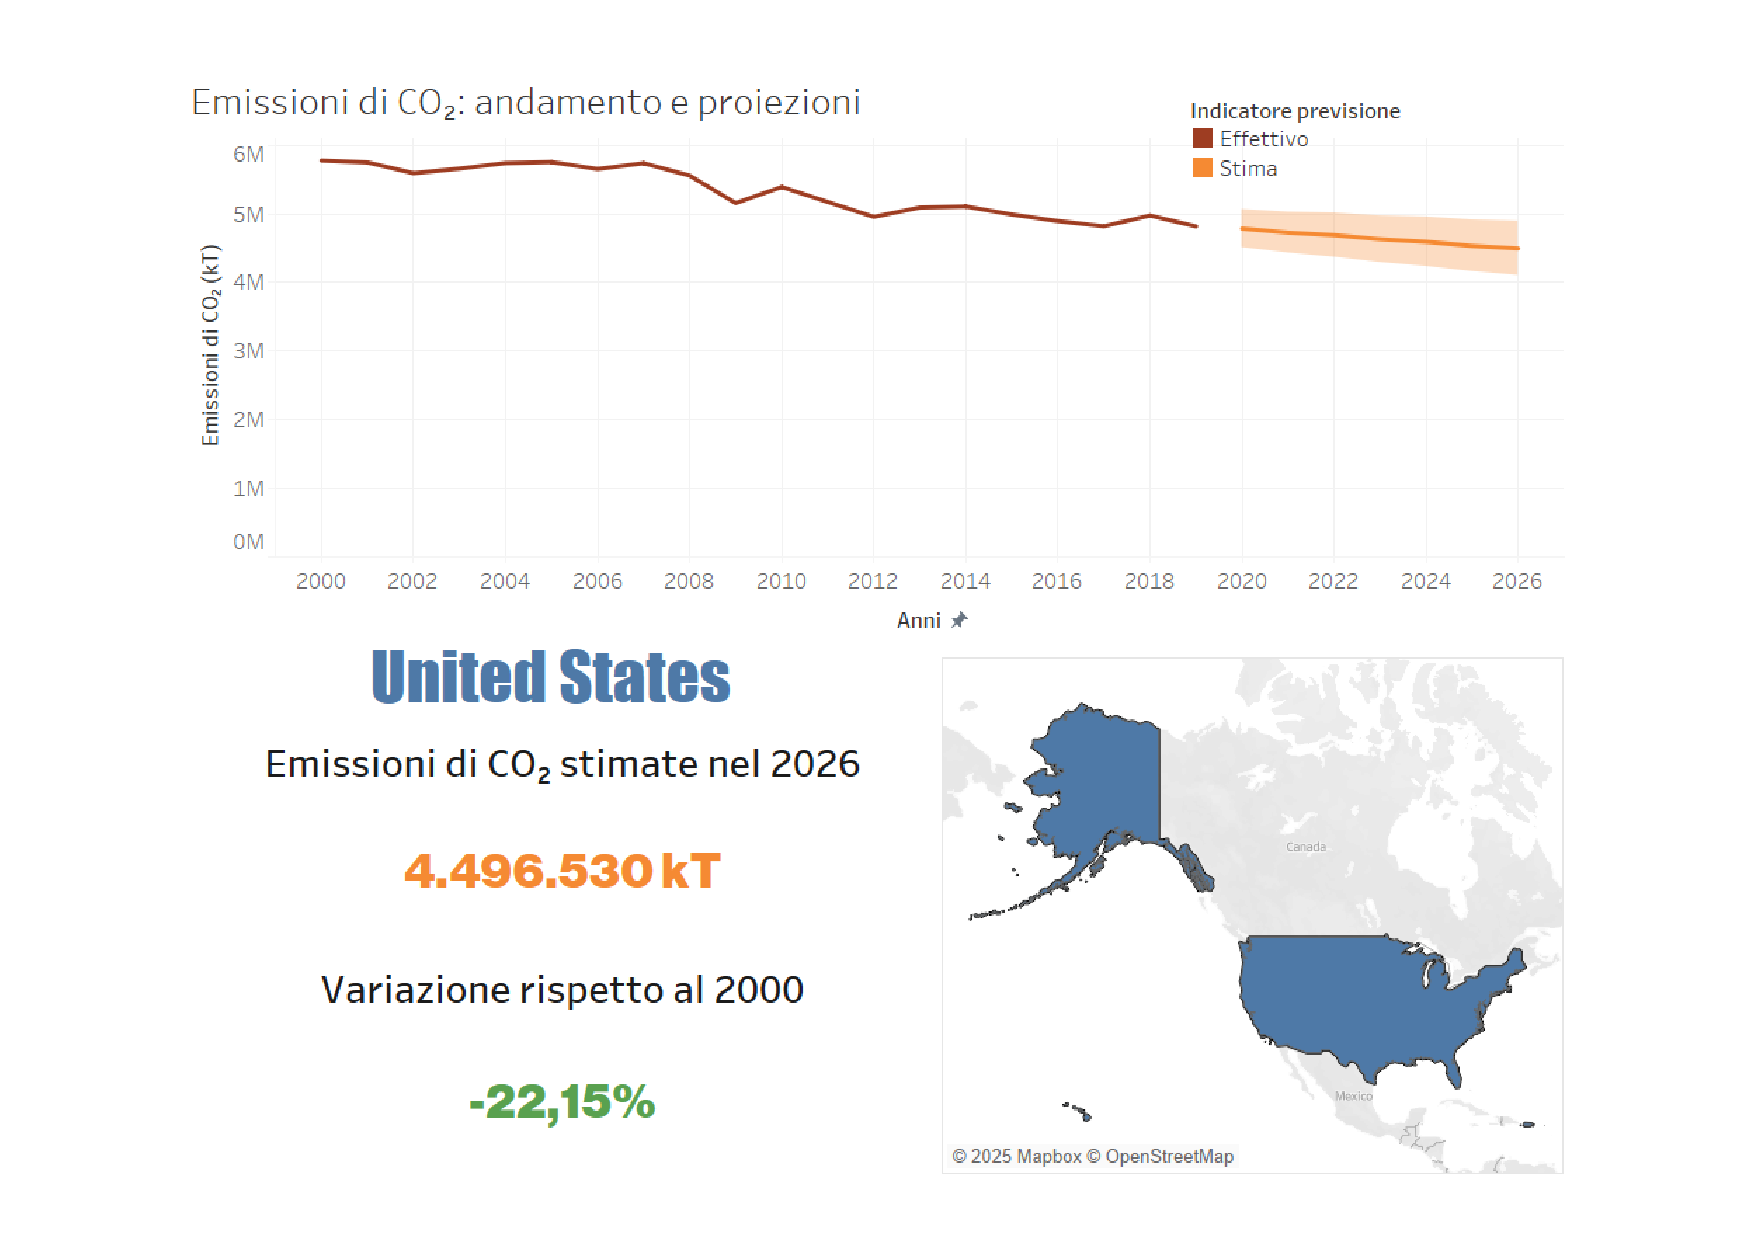
\includegraphics[width=0.7\textwidth]{capitolo_3/img3/previsioni/Dashboard_previsioneCO2_stati_Usa.pdf}}\\
    \subfloat[\textbf{Previsione Cina}]{%
        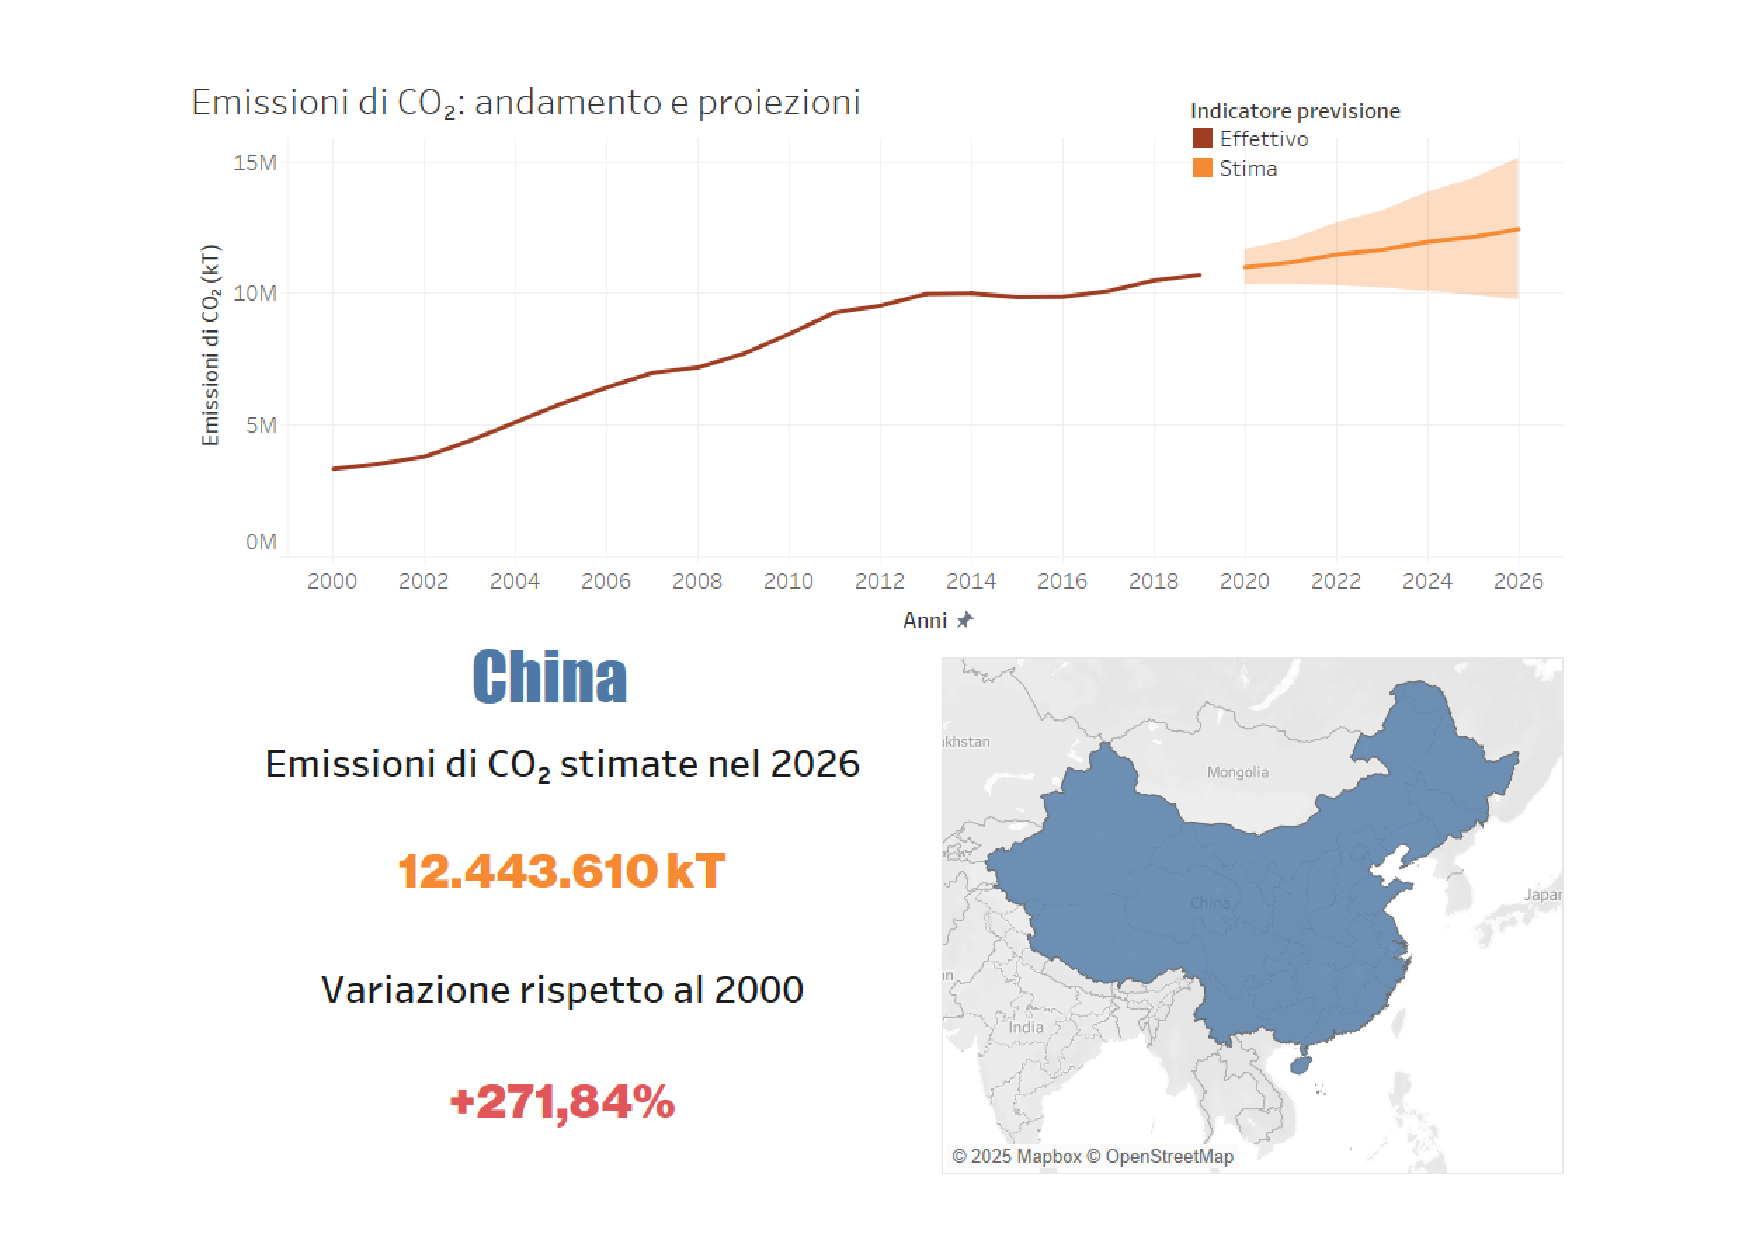
\includegraphics[width=0.7\textwidth]{capitolo_3/img3/previsioni/Dashboard_previsioneCO2_stati_Cina.pdf}} \\
    \subfloat[\textbf{Previsione Italia}]{%
        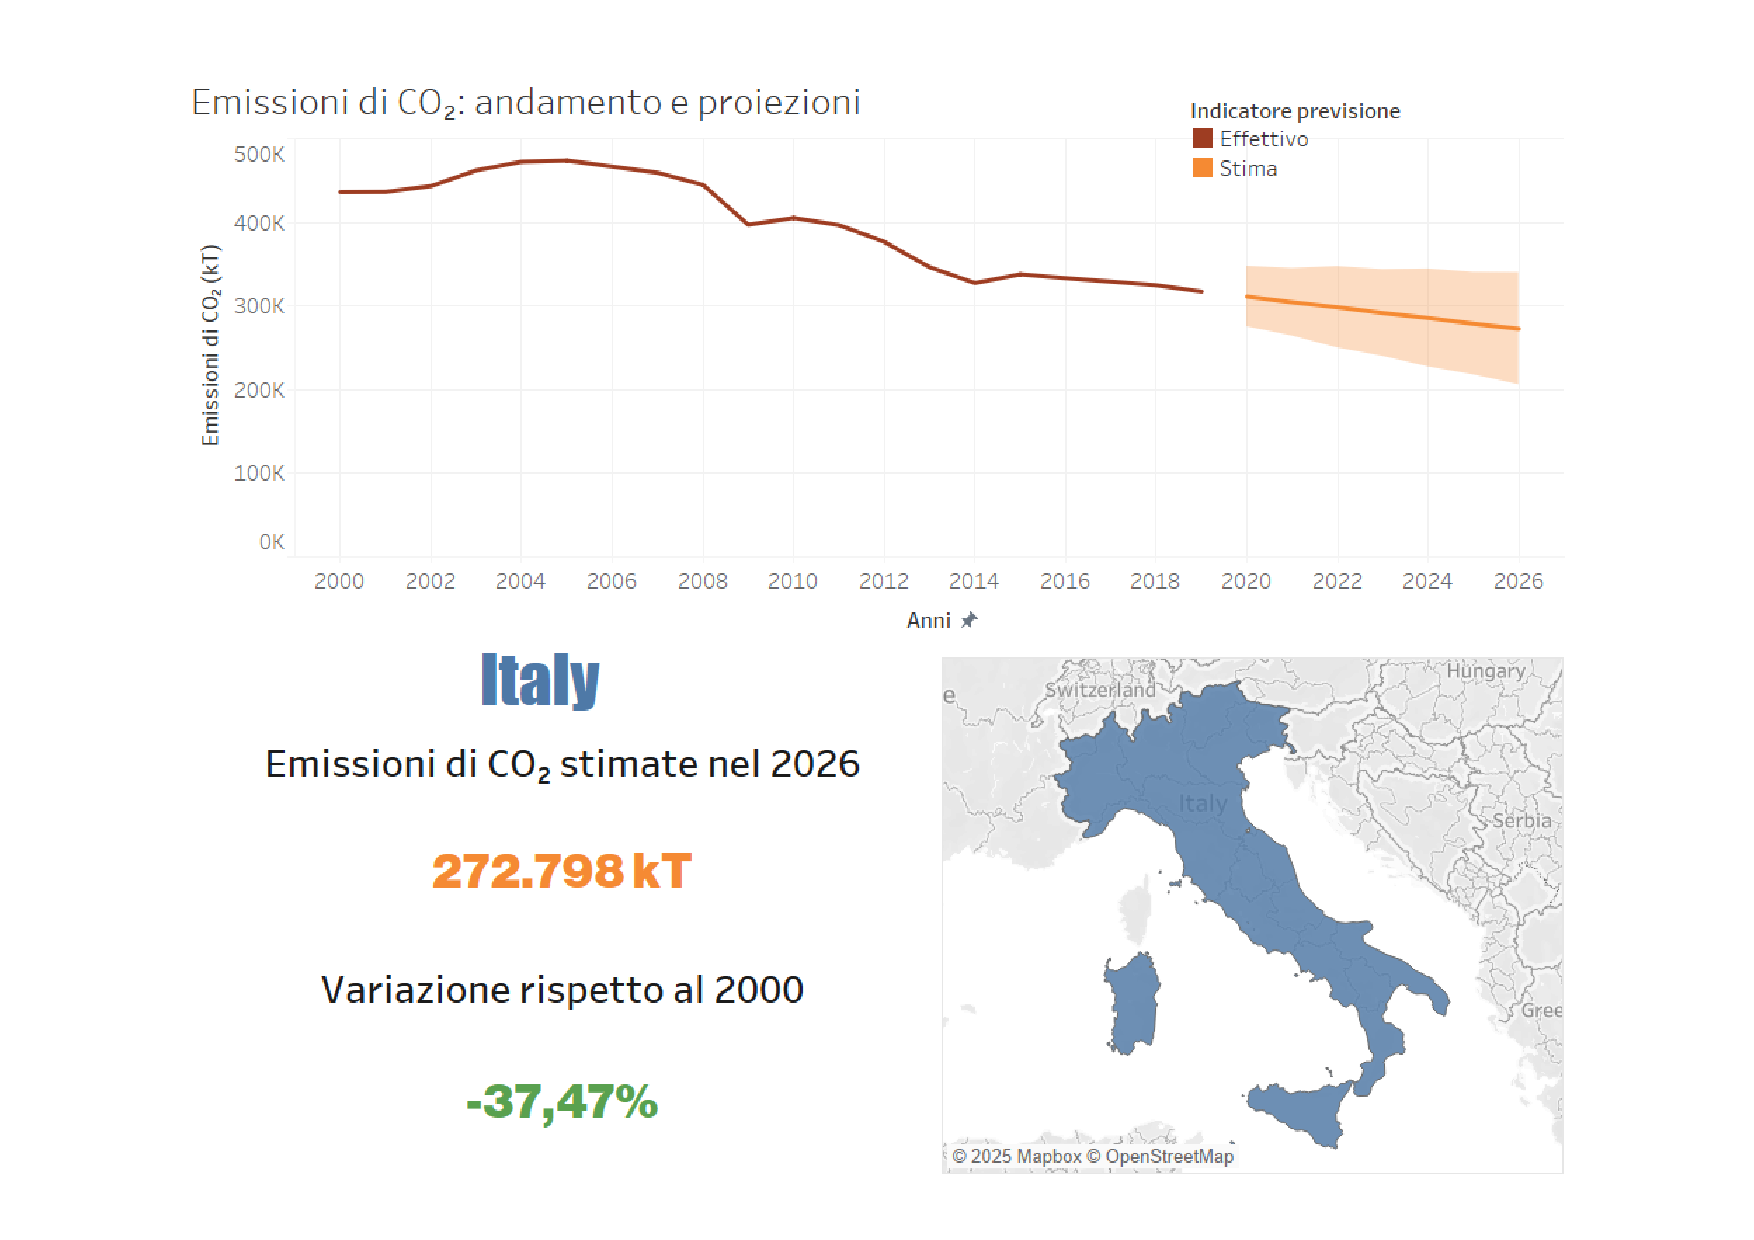
\includegraphics[width=0.7\textwidth]{capitolo_3/img3/previsioni/Dashboard_previsioneCO2_stati_Italia.pdf}}

   \caption{Previsione - Emissioni di CO\textsubscript{2}: andamento e proiezioni - USA, Cina, Italia}
  \label{fig:previsione_1_stati}
\end{figure}

\newpage
\subsection{Previsione - Produzione di elettricità: andamento e previsioni}
La Dashboard illustrata in Figura \ref{fig:previsione_2} presenta l'andamento storico della produzione di elettricità dal 2000 al 2019, integrato con una previsione temporale estesa fino al 2026. I risultati sono suddivisi in tre sezioni, ciascuna dedicata a una specifica tipologia di fonte energetica analizzata nei dataset di riferimento: \textbf{Elettricità da combustibili fossili}, \textbf{Elettricità da energia nucleare} ed \textbf{Elettricità da fonti rinnovabili}.


\begin{figure}[h!]
    \centering
    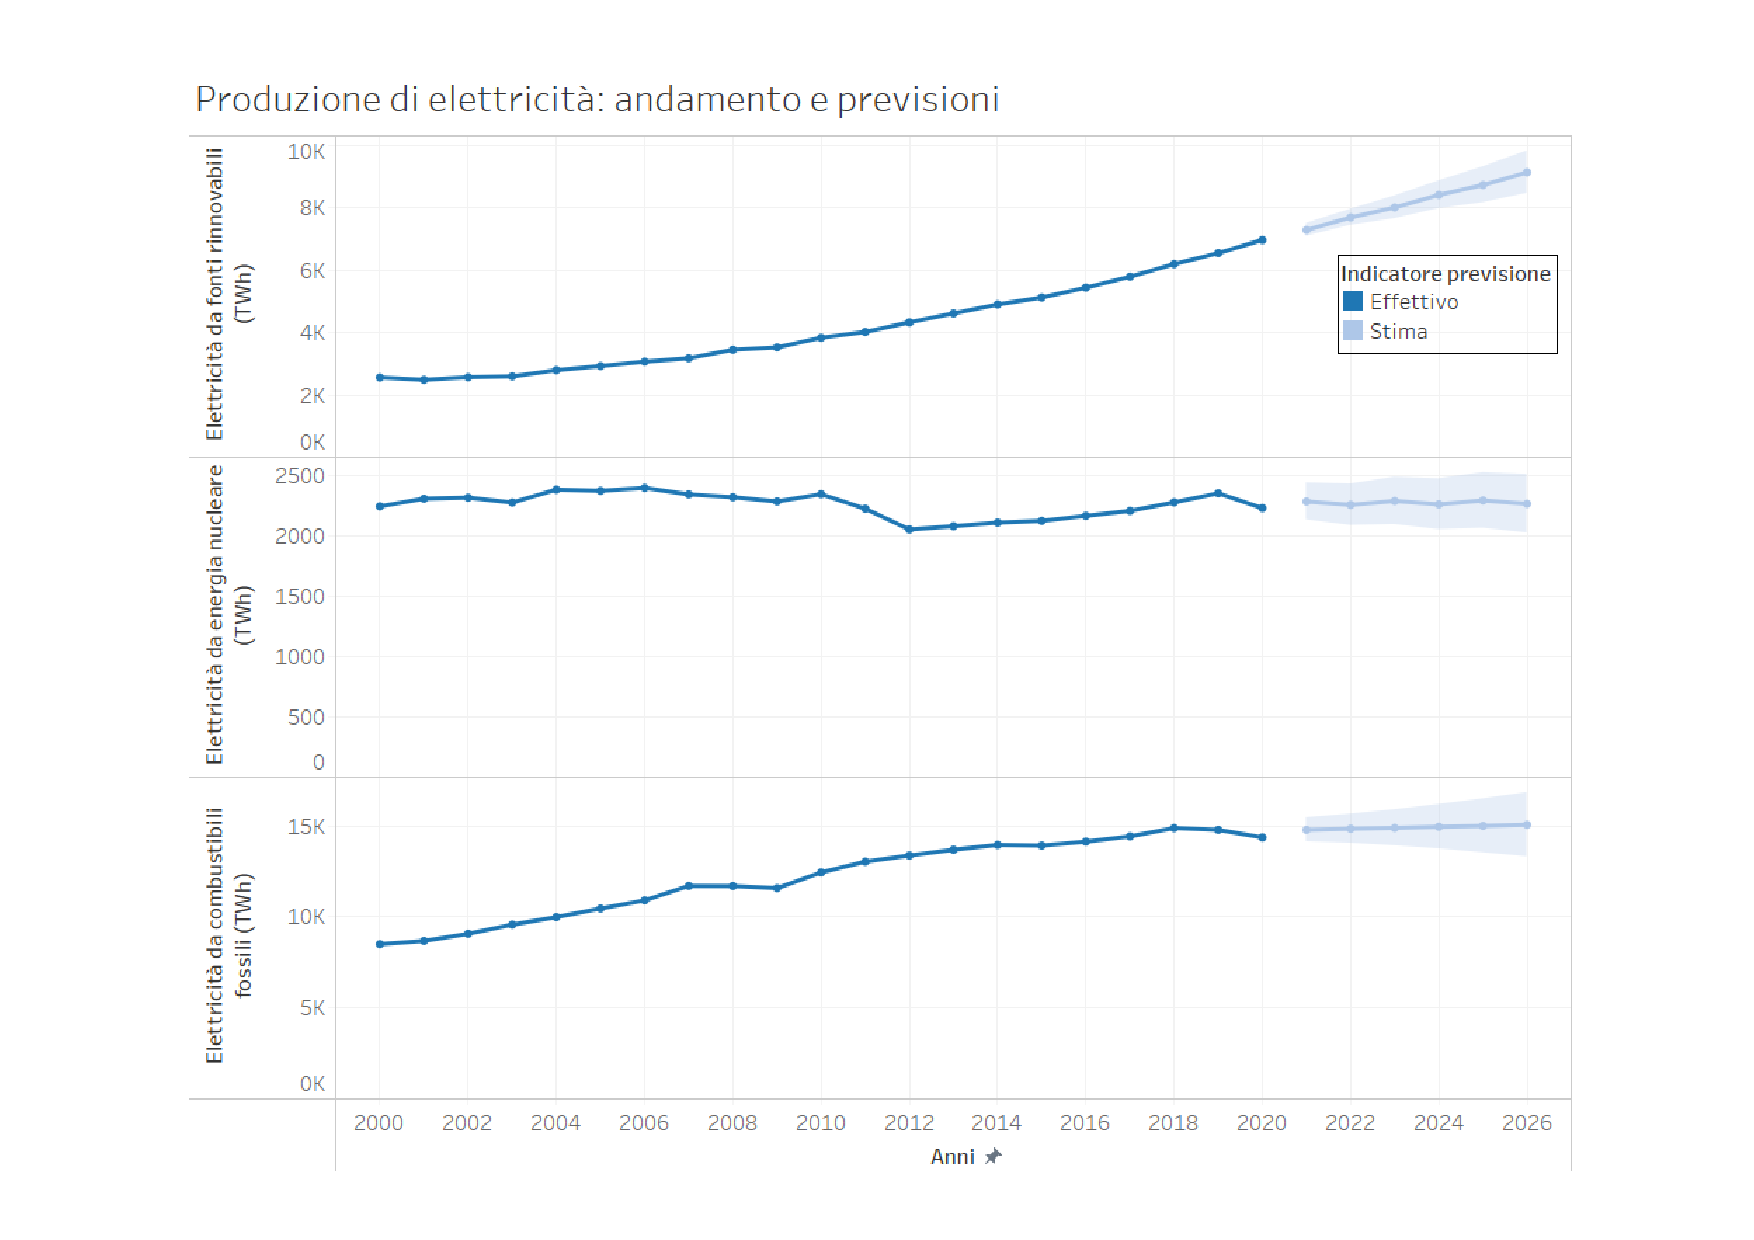
\includegraphics[width=0.98\linewidth]{capitolo_3/img3/previsioni/Dashboard_Previsione_Produzioneelettricità.pdf}
    \caption{Previsione - Produzione di elettricità: andamento e previsioni}
    \label{fig:previsione_2}
\end{figure}

\subsubsection{Risultati della previsione}
Come si può osservare dal grafico riportato in Figura \ref{fig:previsione_2}, la sua struttura è caratterizzata dalle seguenti dimensioni:

\vspace{2mm}
\begin{itemize}
    \item \textit{Asse delle ascisse}: rappresenta l'andamento temporale del fenomeno analizzato, mostrando gli anni dal 2000 al 2026;
    \item \textit{Asse delle ordinate}: indica la quantità di energia prodotta, espressa in terawattora (TWh).
\end{itemize}
\vspace{2mm}


L'analisi si concentra, in particolare, sulle previsioni per il periodo 2020-2026. Dall'osservazione del grafico emergono i seguenti aspetti:

\vspace{2mm}
\begin{itemize}
    \item Per la produzione di elettricità da \textbf{combustibili fossili}, si nota che fino al 2018 c'è stata una crescita costante, seguita da una fase di stabilizzazione. Questo trend si riflette anche nelle previsioni, che indicano valori pressoché invariati nel periodo considerato.
    
    \item Per quanto riguarda l'\textbf{energia nucleare}, la produzione si mantiene stabile sia nei dati storici che nelle previsioni future, senza variazioni significative.
    
    \item La produzione di elettricità da \textbf{fonti rinnovabili} mostra invece una crescita esponenziale, un andamento che continua anche nelle previsioni.
\end{itemize}
\vspace{2mm}

L'analisi del grafico mette in evidenza una chiara distinzione tra le diverse fonti di energia: mentre le fonti tradizionali, come i combustibili fossili e il nucleare, mostrano una tendenza alla stabilità, le energie rinnovabili sono in forte crescita, confermando il loro ruolo sempre più importante nel settore energetico.

Nella Figura \ref{fig:previsione_2_stati} sono riportate le previsioni di produzione di elettricità da fonti rinnovabili, suddivise per ciascuno Stato analizzato\footnote{La selezione degli Stati, ovvero Stati Uniti, Cina e Italia, è stata effettuata sulla base delle analisi precedenti, al fine di consentire un confronto più diretto e significativo.}.

La struttura delle Dashboard è articolata nei seguenti elementi:

\vspace{2mm}
\begin{itemize}
\item \textit{Grafico a linee}: rappresentazione grafica dell'andamento previsto della produzione di elettricità da fonti rinnovabili;
\item \textit{Mappa geografica}: visualizzazione geografica dello Stato di riferimento;
\item \textit{KPI}: parametri che includono il nome dello Stato, la previsione della produzione da fonti rinnovabili per l'anno 2026 espressa in termini percentuali, e la variazione rispetto al valore registrato nel 2000, espressa sempre in percentuale.
\end{itemize}
\vspace{2mm}

Si osserva come, per tutti e tre gli Stati considerati, la produzione di elettricità da fonti rinnovabili abbia registrato una crescita costante a partire dal 2000. Le previsioni effettuate riflettono tale tendenza, suggerendo il mantenimento di un incremento progressivo nel futuro.

\begin{figure}[p]
    \centering
    \subfloat[\textbf{Previsione USA}]{%
        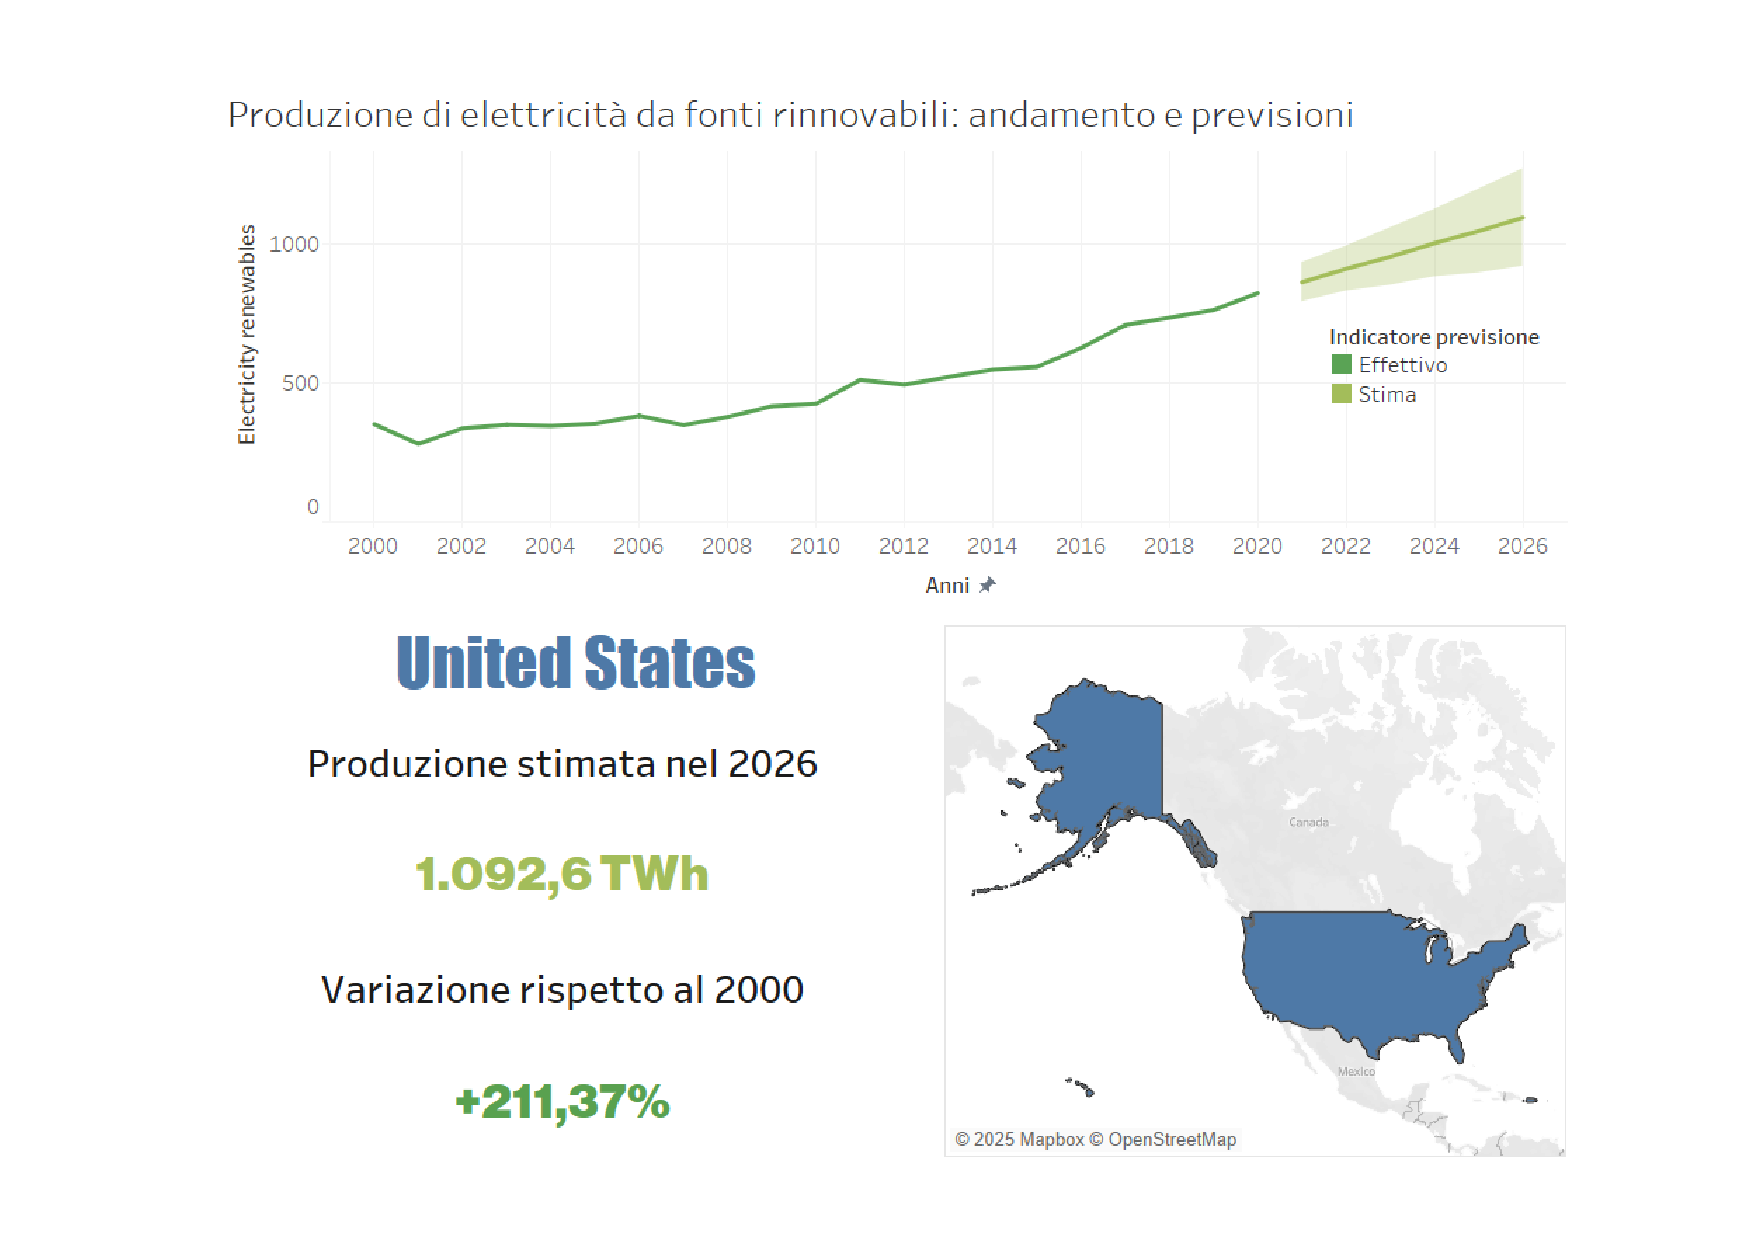
\includegraphics[width=0.7\textwidth]{capitolo_3/img3/previsioni/Dashboard_previsionerinnovabile_stati_Usa.pdf}}\\
    \subfloat[\textbf{Previsione Cina}]{%
        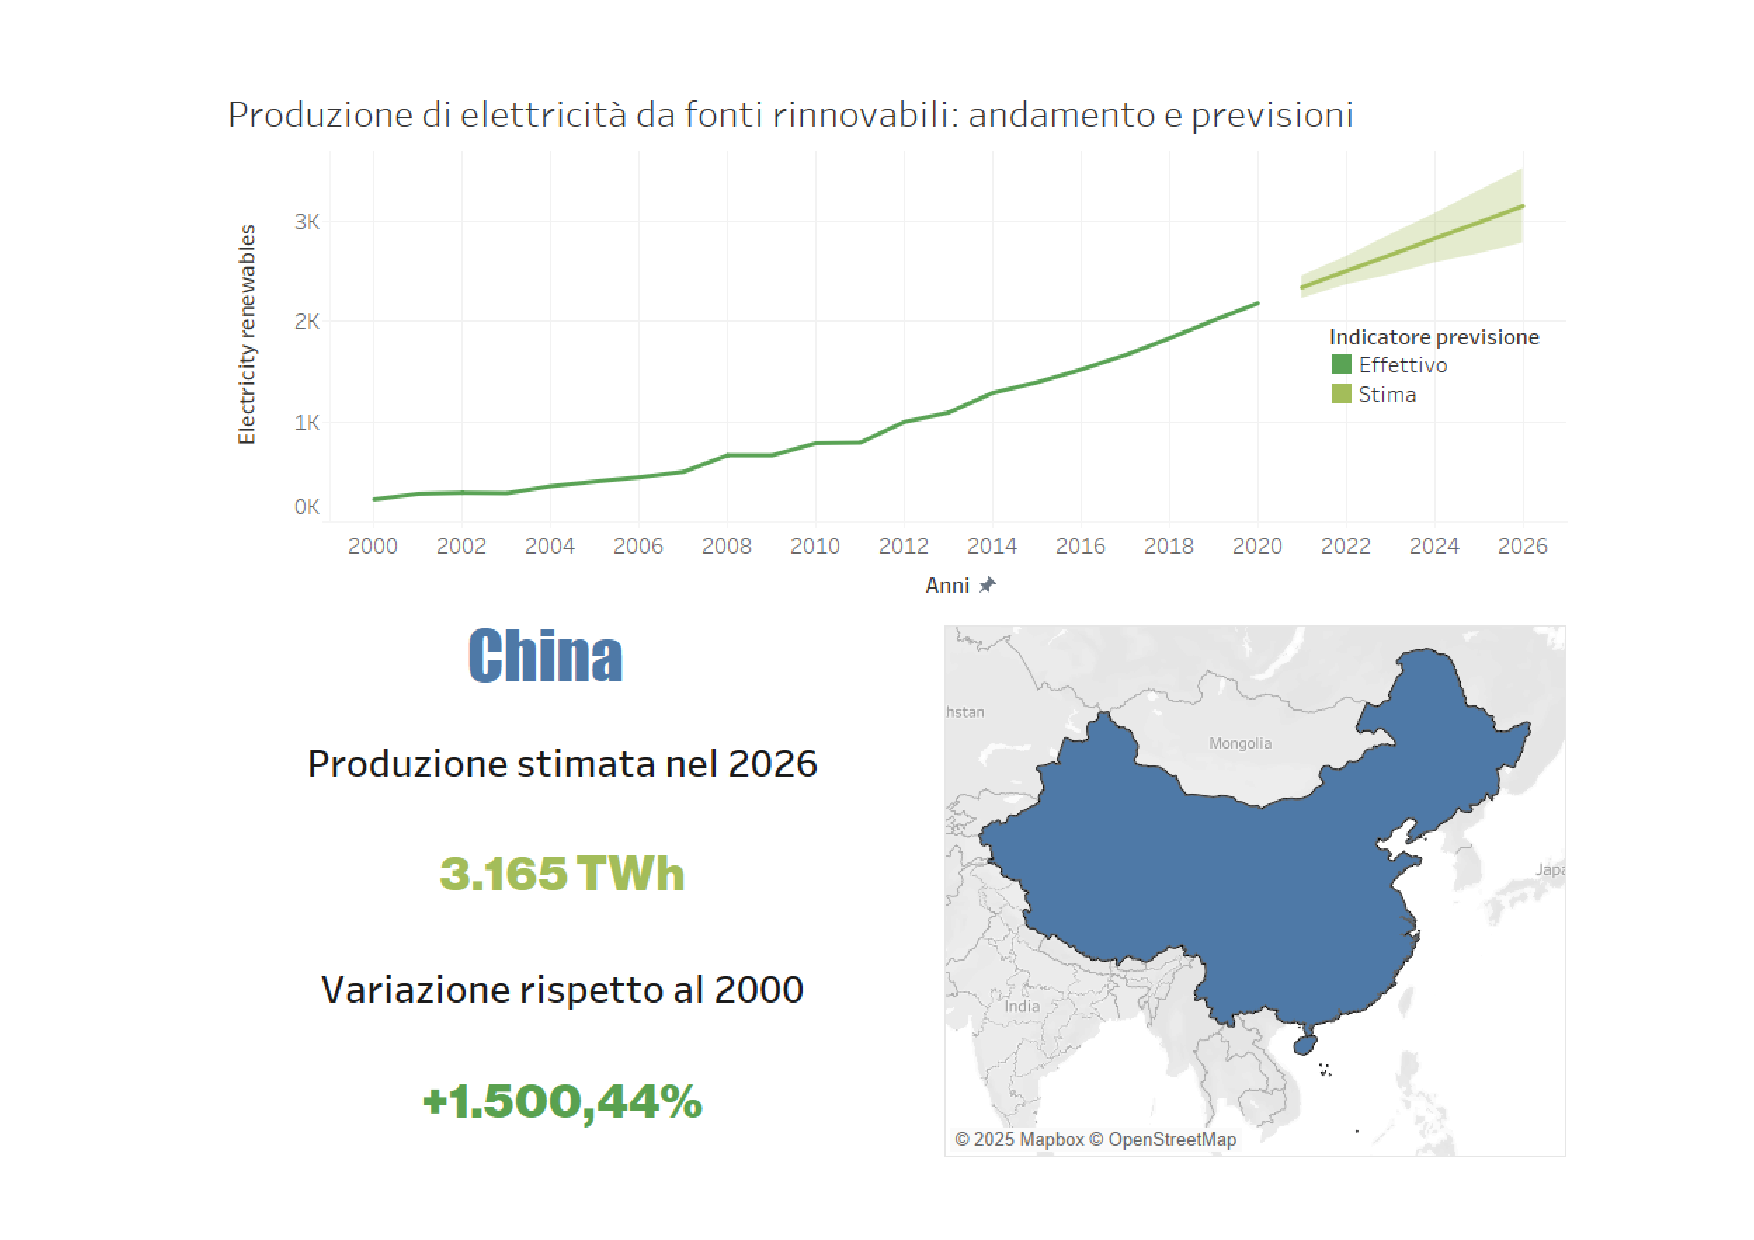
\includegraphics[width=0.7\textwidth]{capitolo_3/img3/previsioni/Dashboard_previsionerinnovabile_stati_Cina.pdf}} \\
    \subfloat[\textbf{Previsione Italia}]{%
        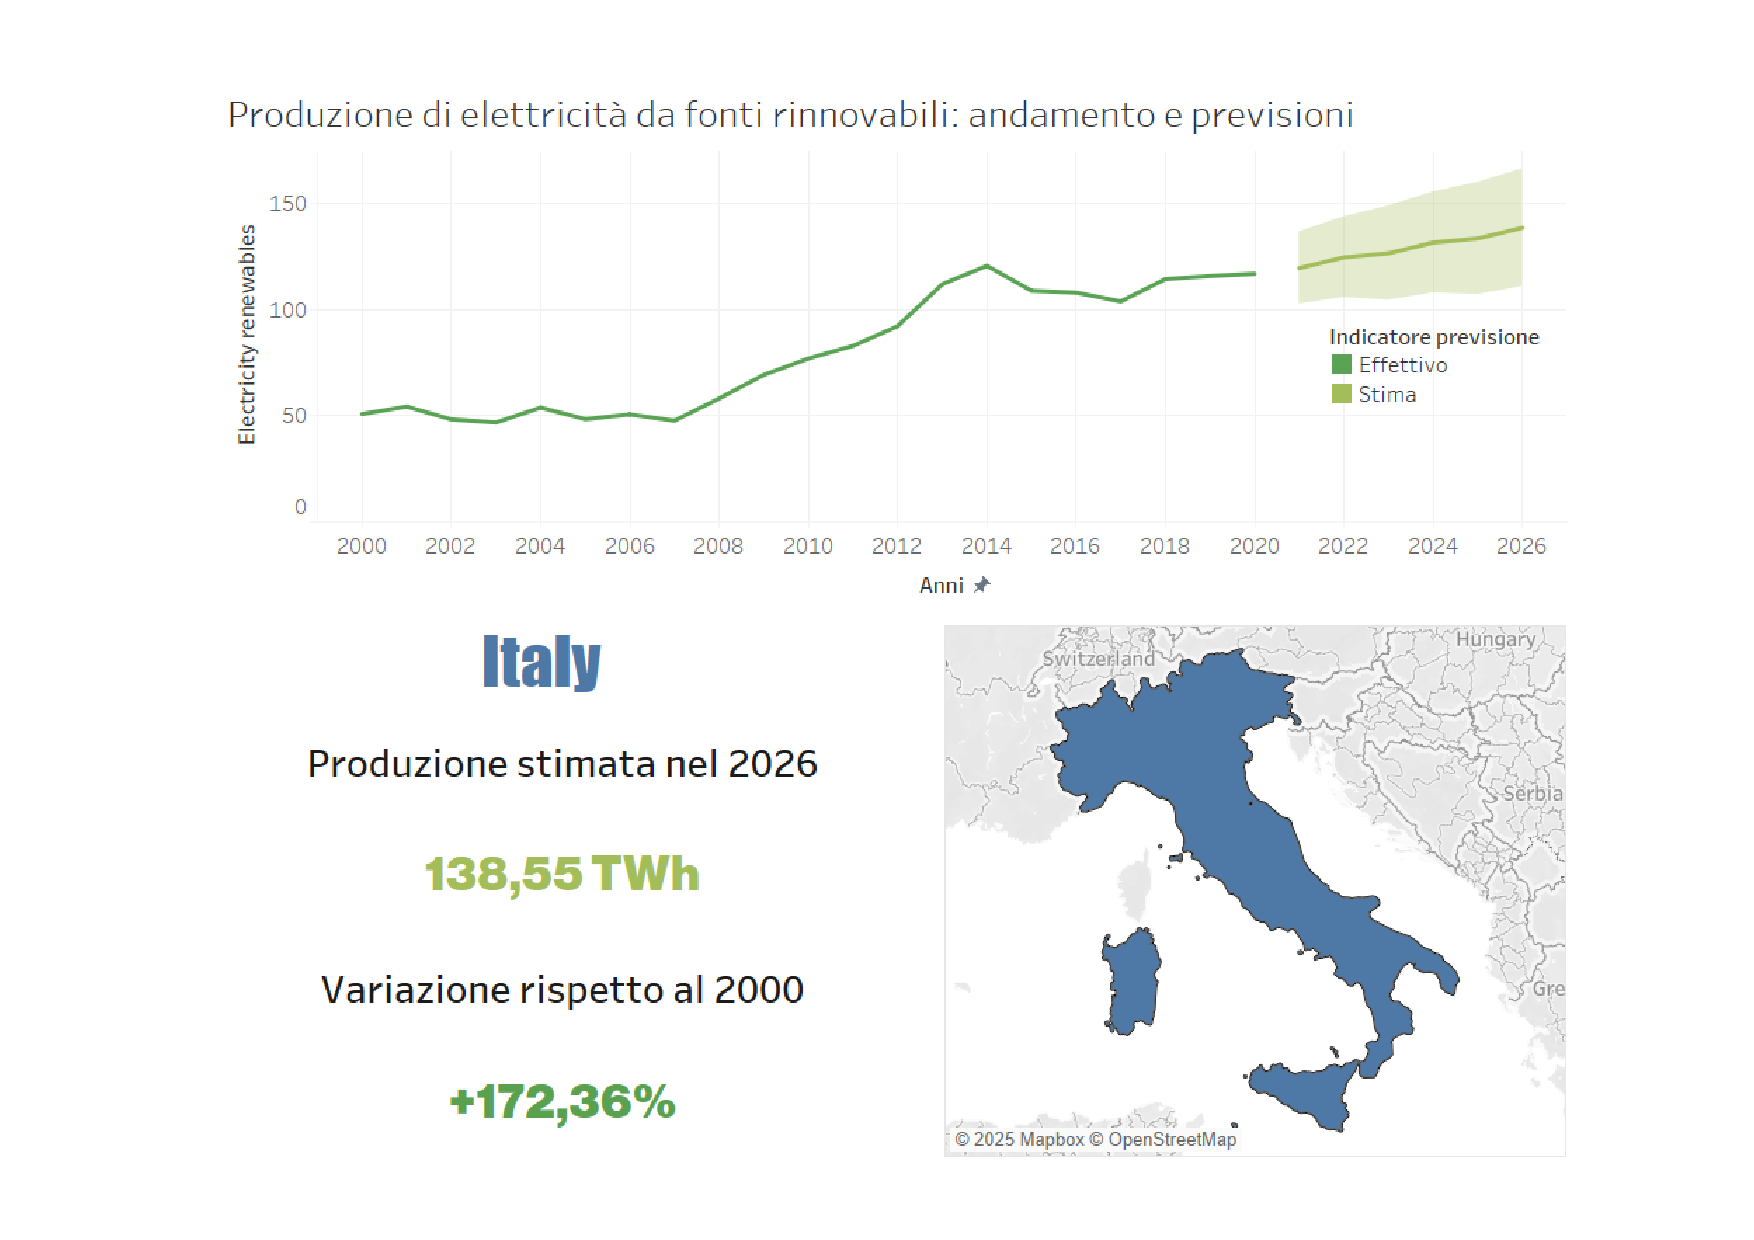
\includegraphics[width=0.7\textwidth]{capitolo_3/img3/previsioni/Dashboard_previsionerinnovabile_stati_Italia.pdf}}

   \caption{Previsione - Produzione di elettricità: andamento e previsioni - USA, Cina, Italia}
  \label{fig:previsione_2_stati}
\end{figure}

\newpage
\subsection{Previsione - Variazione di temperatura: andamento e proiezioni}
La Dashboard mostrata in Figura \ref{fig:previsione_3} illustra le variazioni di temperatura dal 2000 al 2019, integrato con una previsione temporale estesa fino al 2026. Il grafico integra diverse descrizioni che agevolano l'utente nella comprensione dei punti critici del grafico. 

\begin{figure}[h!]
    \centering
    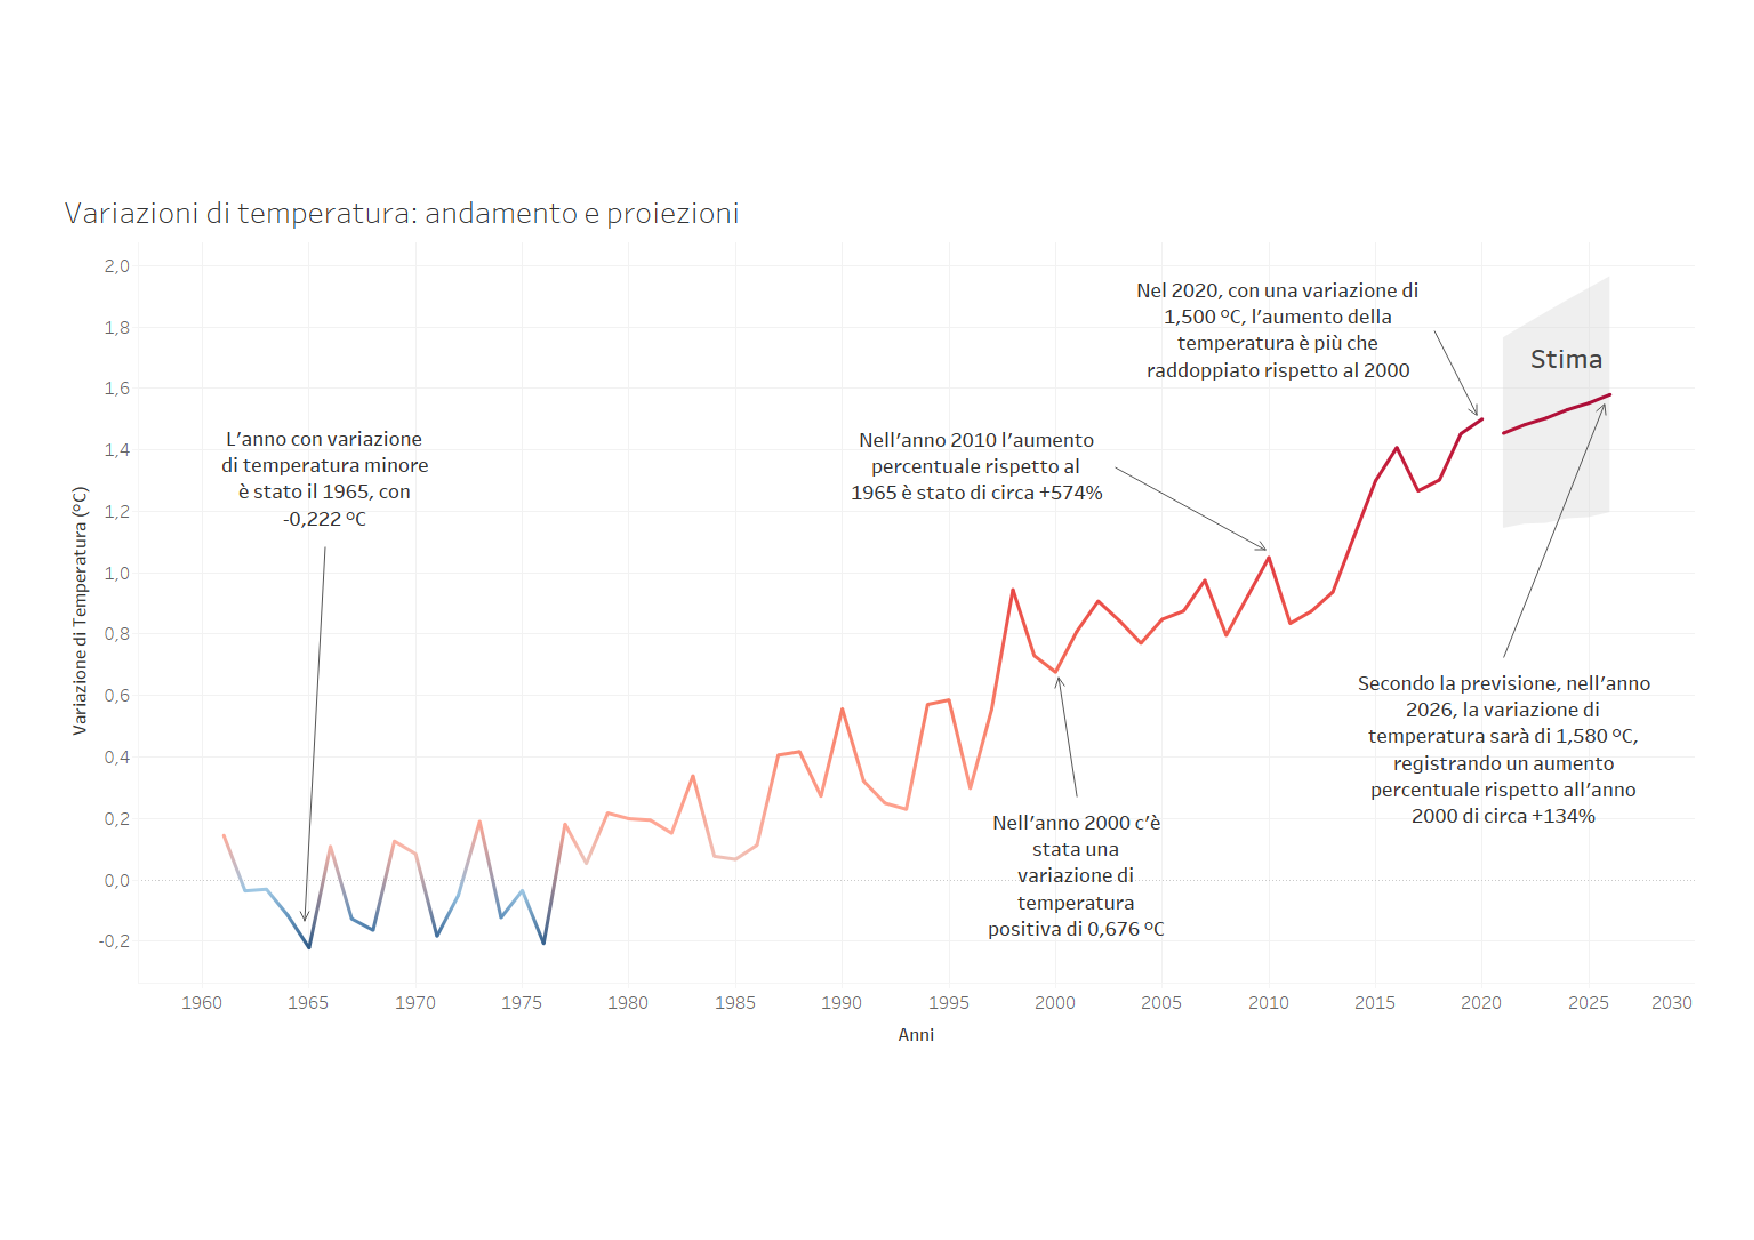
\includegraphics[width=0.98\linewidth]{capitolo_3/img3/previsioni/Dashboard_Previsione_Temperatura.pdf}
    \caption{Previsione - Variazione di temperatura: andamento e proiezioni}
    \label{fig:previsione_3}
\end{figure}


\subsubsection{Risultati della previsione}
Come illustrato nel grafico riportato in Figura \ref{fig:previsione_3}, la sua struttura è caratterizzata dalle seguenti componenti:

\vspace{2mm}
\begin{itemize}
\item \textit{Asse delle ascisse}: rappresenta l'andamento temporale del fenomeno analizzato, coprendo il periodo dal 2000 al 2026;
\item \textit{Asse delle ordinate}: indica la variazione della temperatura, espressa in gradi Celsius (°C).
\end{itemize}
\vspace{2mm}

L'analisi si concentra in particolare sulle previsioni relative al periodo 2020-2026. Come evidenziato dalle annotazioni presenti nel grafico, la previsione per il 2026 indica una variazione di temperatura pari a 1,580°C, corrispondente a un incremento percentuale di circa +134\% rispetto al valore registrato nel 2000.

Nelle Figure \ref{fig:previsione_3_stati} sono riportati i risultati delle previsioni sulle variazioni di temperatura, suddivisi per ciascuno degli Stati analizzati, ovvero Stati Uniti, Cina e Italia, come effettuato per le precedenti previsioni.  

Dall'osservazione dei dati emerge, per tutti e tre gli Stati considerati, una tendenza all'aumento della temperatura nel periodo esaminato. Questo andamento crescente suggerisce un'evoluzione costante del fenomeno, confermando le dinamiche già individuate nelle analisi precedenti.


\begin{figure}[p]
    \centering
    \subfloat[\textbf{Previsione USA}]{%
        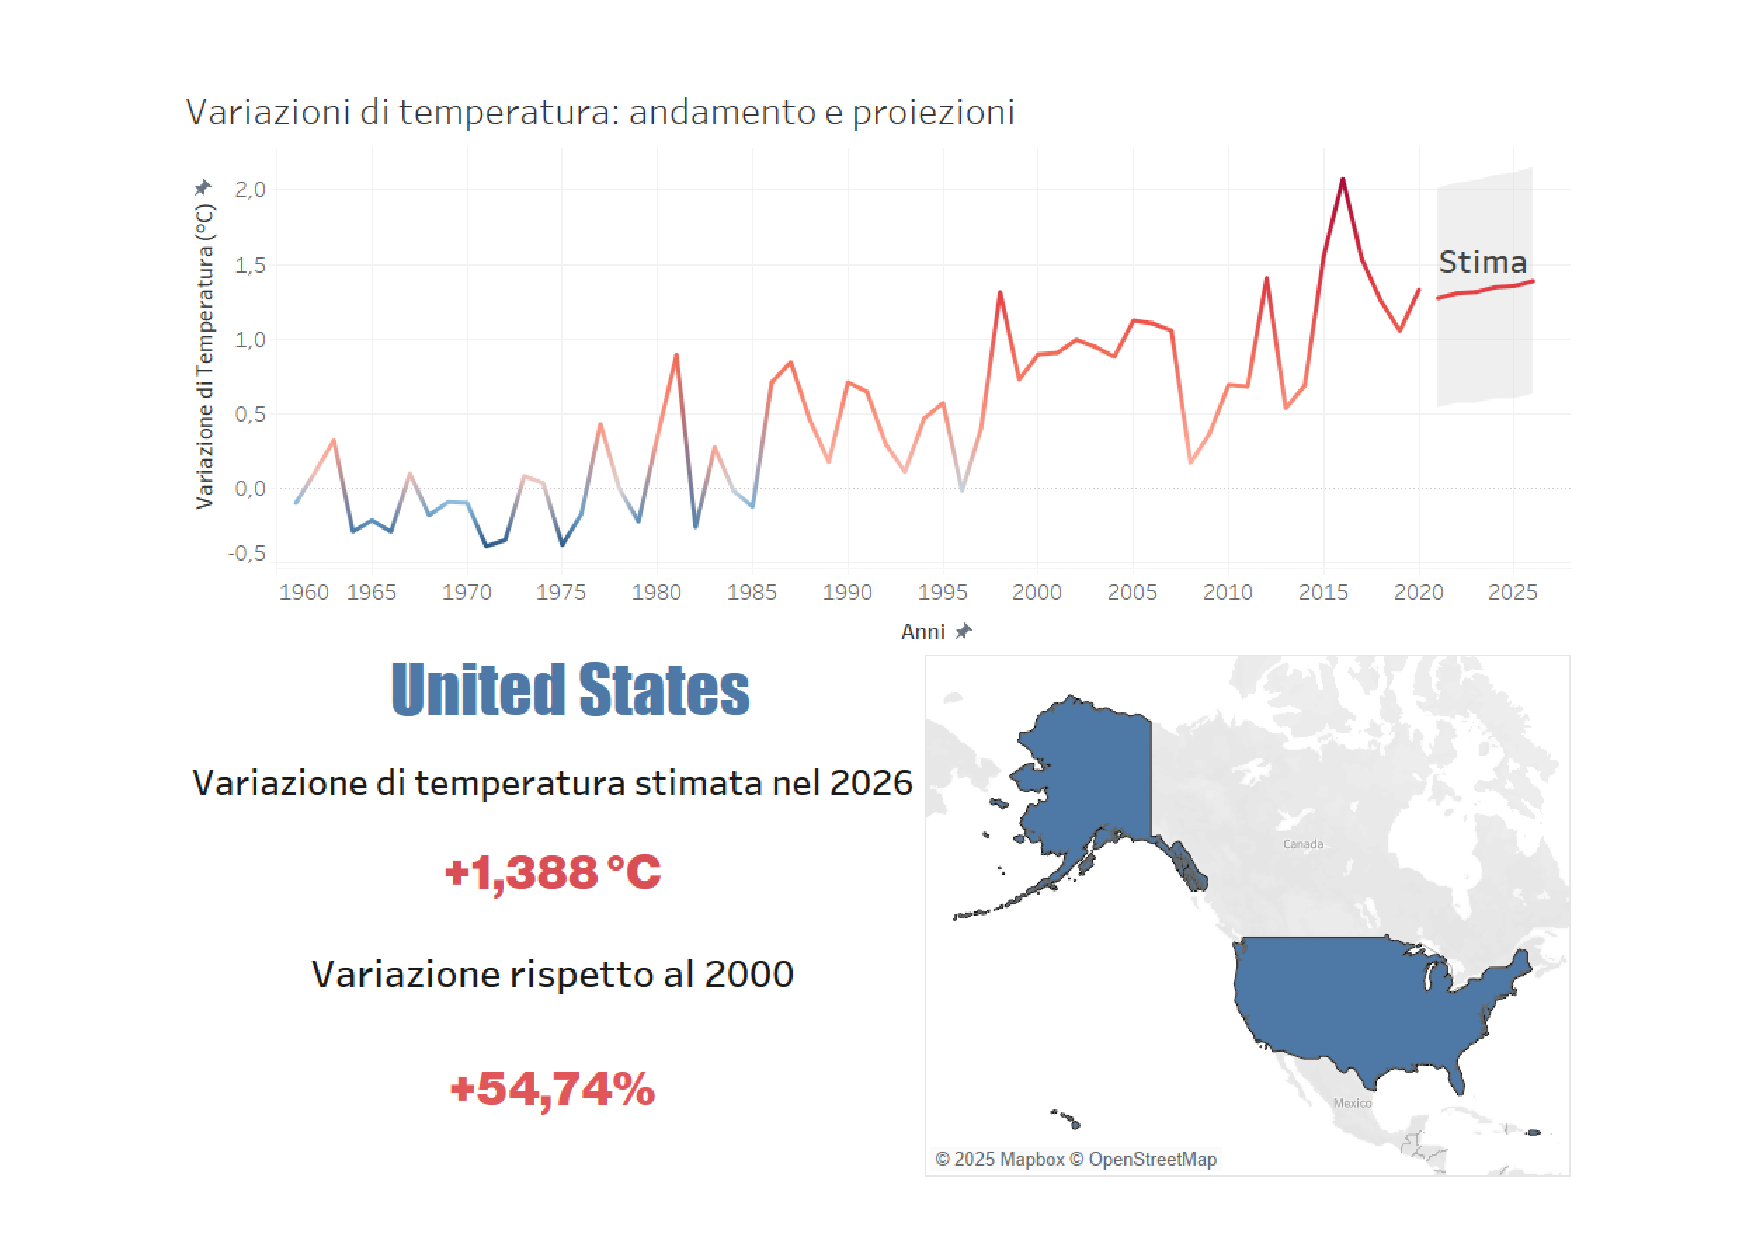
\includegraphics[width=0.7\textwidth]{capitolo_3/img3/previsioni/Dashboard_previsionetemperatura_stati_Usa.pdf}}\\
    \subfloat[\textbf{Previsione Cina}]{%
        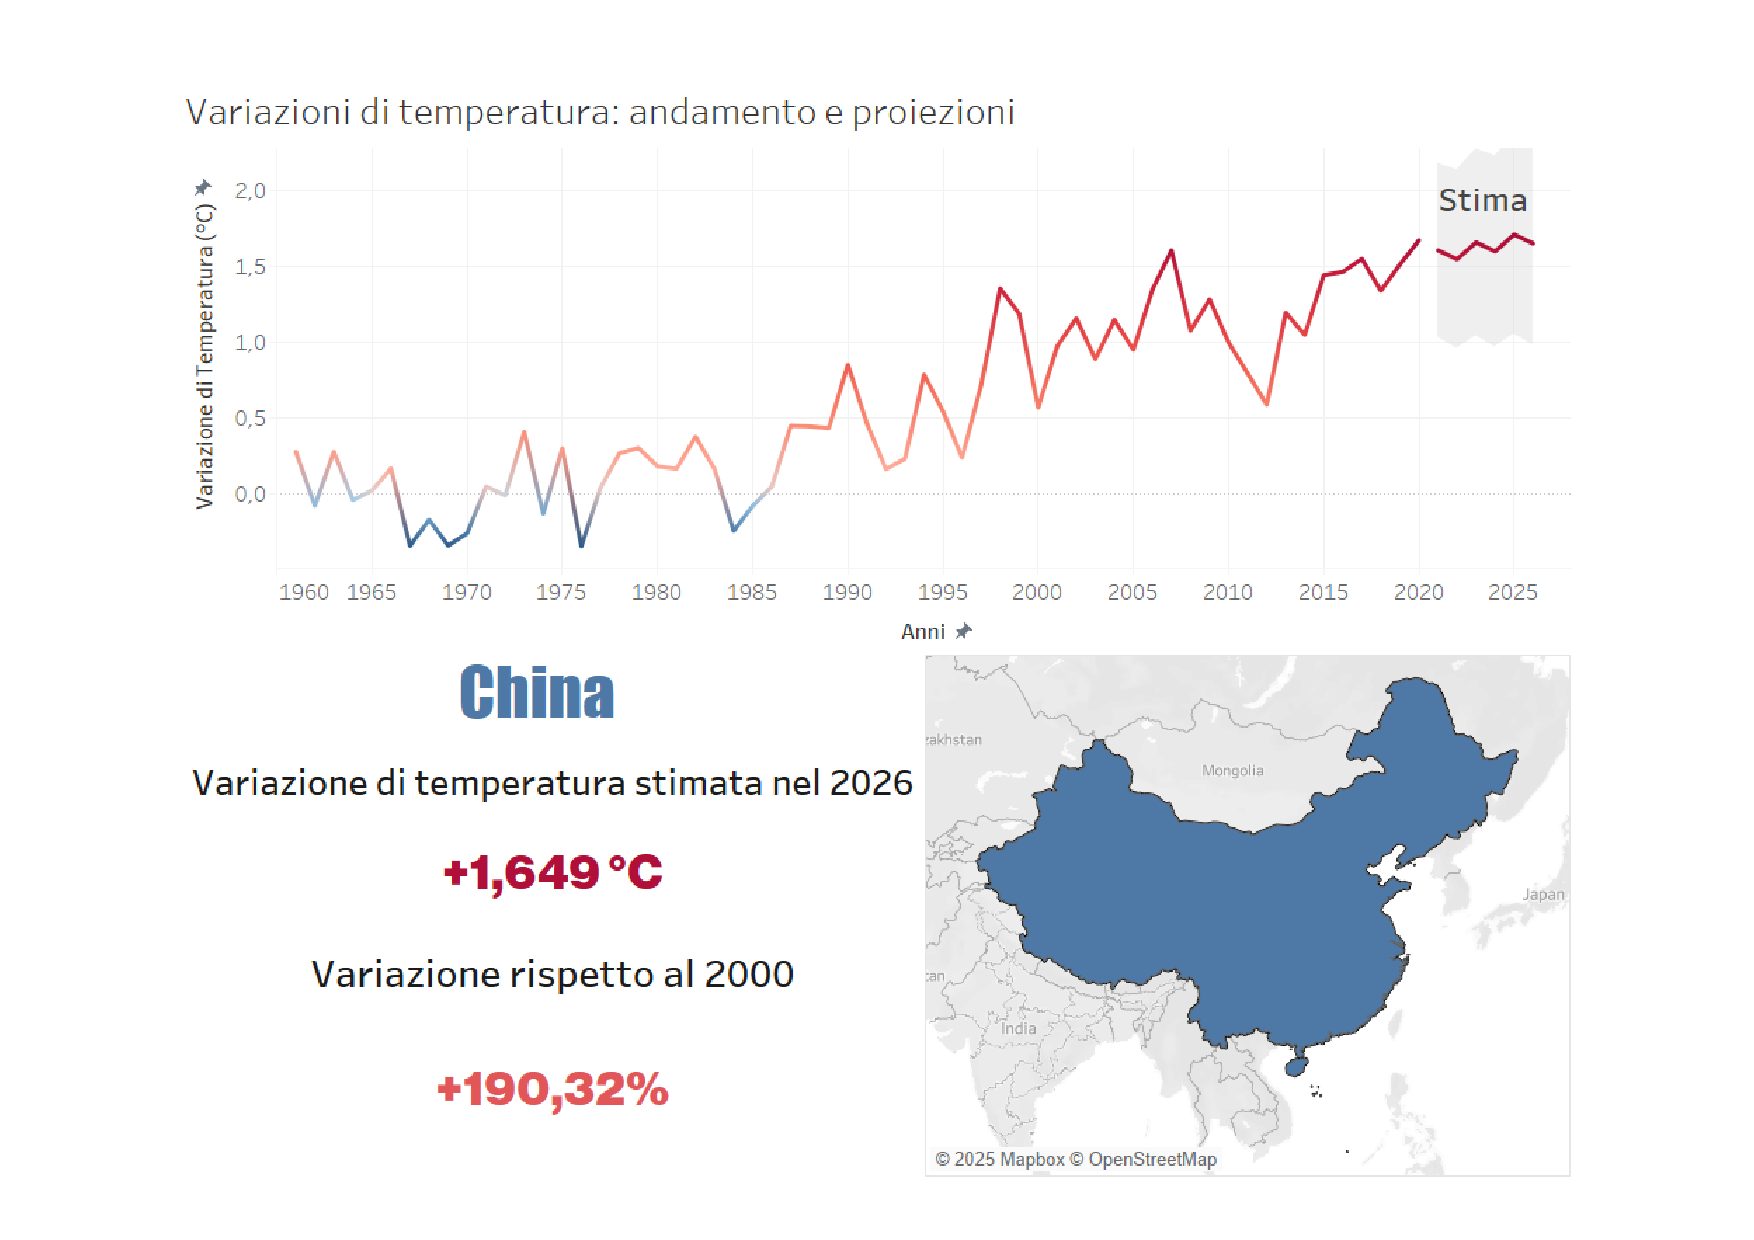
\includegraphics[width=0.7\textwidth]{capitolo_3/img3/previsioni/Dashboard_previsionetemperatura_stati_China.pdf}} \\
    \subfloat[\textbf{Previsione Italia}]{%
        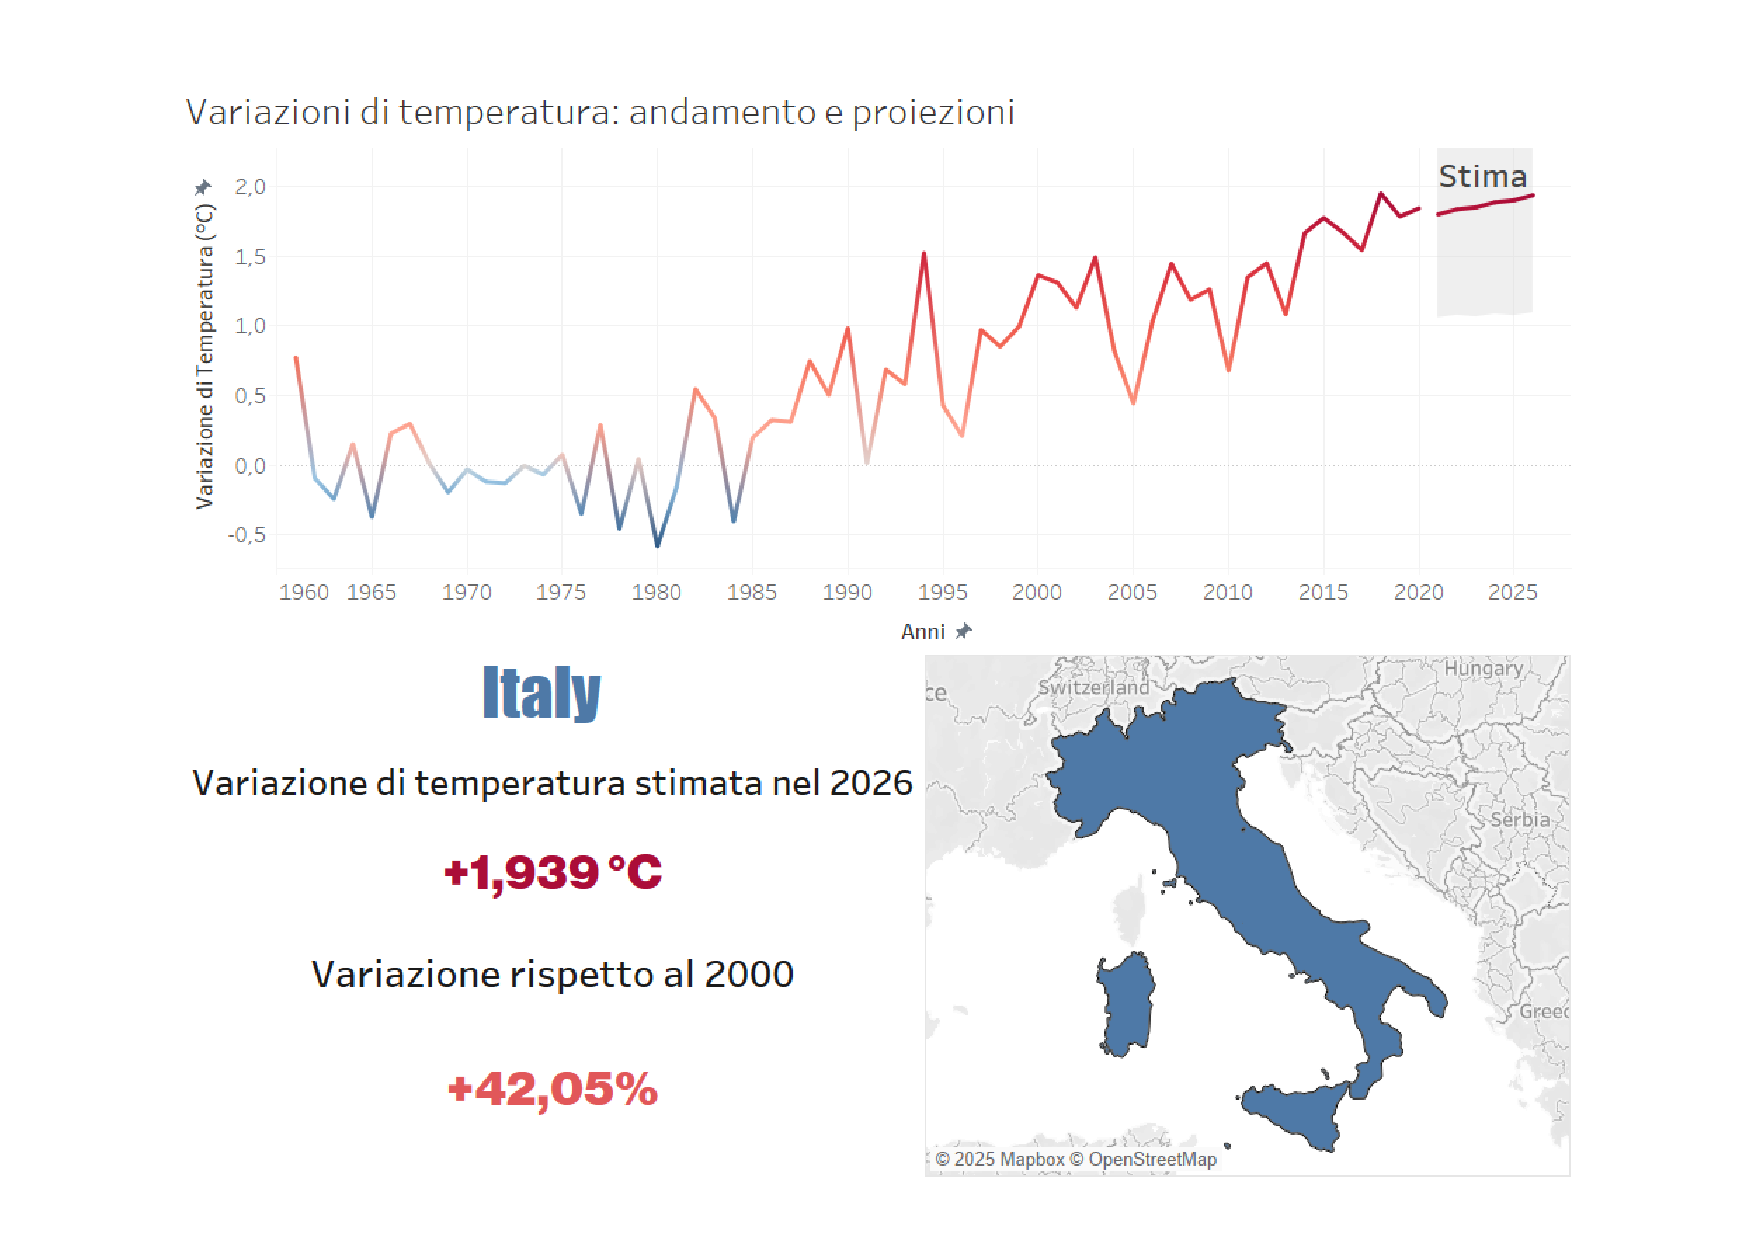
\includegraphics[width=0.7\textwidth]{capitolo_3/img3/previsioni/Dashboard_previsionetemperatura_stati_Italia.pdf}}

   \caption{Previsione - Variazione di temperatura: andamento e proiezioni - USA, Cina, Italia}
  \label{fig:previsione_3_stati}
\end{figure}

